\documentclass[galley,usenatbib]{mn2e}
%\documentclass[twocolumn,galley]{mn2e}
%\documentclass[onecolumn,galley,draft]{mn2e}
\usepackage{myaasmacros}
\usepackage{mathrsfs}
\usepackage{amsmath}
\usepackage{graphicx}

\def\newblock{\hskip .11em plus .33em minus .07em}

\newcommand{\Glass}{{\sc Glass}}
\newcommand{\PixeLens}{{\sc PixeLens}}
\newcommand{\Rmap}{\ensuremath{R_\mathrm{map}}}
\newcommand{\Rpix}{\ensuremath{R_\mathrm{pix}}}
\newcommand{\M}{\ensuremath{\mathscr{M}}}
\newcommand{\E}{\ensuremath{\mathscr{E}}}
\newcommand{\eps}{\ensuremath{\varepsilon}}

\newcommand{\Eavg}{\ensuremath{\langle \E \rangle}}

\newcommand{\kpc}{\ensuremath{\mathrm{kpc}}}
\newcommand{\Msun}{\ensuremath{\mathrm{M}_\odot}}
\newcommand{\tabref}[1] {Table~\ref{#1}}
\newcommand{\figref}[1] {Figure~\ref{#1}}
\newcommand{\eqnref}[1] {Eq.~(\ref{#1})}
\newcommand{\secref}[1] {\S\ref{#1}}
\newcommand{\appref}[1] {Appendix~\ref{#1}}
\newcommand{\e}[1]{\ensuremath{\times 10^{#1}}}
\renewcommand{\vec}[1]{\ensuremath{\boldsymbol{#1}}}

% From aastex.cls
\newcommand\plotone[1]{%
 \centering
 \leavevmode
 \includegraphics[width={\columnwidth}]{#1}%
}%
\newcommand\plottwo[2]{{%
 \centering
 \leavevmode
 \columnwidth=.45\columnwidth
 \includegraphics[width={\columnwidth}]{#1}%
 \hfil
 \includegraphics[width={\columnwidth}]{#2}%
}}%
\newcommand\plotthree[3]{{%
 \centering
 \leavevmode
 \columnwidth=.30\columnwidth
 \includegraphics[width={\columnwidth}]{#1}%
 \hfil
 \includegraphics[width={\columnwidth}]{#2}%
 \hfil
 \includegraphics[width={\columnwidth}]{#3}%
}}%


\title[\Glass]{Gravitational Lens Recovery with \Glass: How to measure the mass profile and shape of a lens}
\author{%
Jonathan P. Coles 
\and 
Justin I. Read
\and 
Prasenjit Saha 
}

\begin{document}
\maketitle

\begin{abstract}
We use a new non-parametric gravitational -- \Glass -- to determine what quality of data (strong lensing, stellar kinematics, and/or stellar masses) are required to measure the circularly averaged mass profile of a lens and its shape. \Glass\ uses an under-constrained adaptive grid of mass pixels to model the lens, searching through thousands of models to marginalise over model uncertainties. Our key findings are as follows: (i) for pure lens data, multiple sources with wide redshift separation give the strongest constraints as this breaks the well-known mass-sheet or steepness degeneracy; (ii) a single quad with time delays also performs well, giving a good recovery of both the mass profile and its shape; (iii) stellar masses -- for lenses where the stars dominate the central potential -- can also break the steepness degeneracy, giving a recovery almost as good as having time delay data or multiple source redshifts; (iv) stellar kinematics are similarly powerful if the data extend beyond the half light radius of the stars $r \gg r_{1/2}$ (required to integrate out the effect of the unknown velocity anisotropy, $\beta(r)$); and (v) if the lensing data already probe the mass profile over the region $r \sim r_{1/2}$, then stellar kinematic data can be used to probe $\beta(r)$ -- an interesting dynamic quantity in its own right. Where information on the mass distribution from lensing and other probes becomes redundant, this opens up the possibility of using strong lensing to constrain cosmological models. We will study this, and present the first results from \Glass\ applied to real data, in forthcoming papers.
\end{abstract}

%(Linear constraints are applied simultaneously with the lens constraints; non-linear constraints are applied in post-processing, with models accepted or rejected based on their likelihood.) 
%These are quantities of key interest for probing the dark matter distribution in galaxies and galaxy clusters to test galaxy formation models and cosmology.

\section{Introduction}\label{sec:intro} %-----------------------------------------------------
Since the discovery of the first gravitational lens
\citep{1979Natur.279..381W}, lensing has become an increasingly important probe
of the distribution of mass in the Universe
\citep{1937ApJ....86..217Z,2012arXiv1206.1225A}. Strong lensing in particular 
provides a powerful probe of the mass distribution at the heart of galaxies and
galaxy clusters \citep{2010CQGra..27w3001B,2007ApJ...667..645R,2006ApJ...652L...5S,2009ApJ...690..154S}, giving valuable constraints on the nature of dark matter \citep{2006ApJ...652L...5S,2013ApJ...765...25N}, cosmology 
\citep{2010Sci...329..924J, 2008ApJ...679...17C}, and galaxy formation \citep{2012MNRAS.424..104L}. To date, some $\sim$400 strong lenses are
known\footnote{{\tt http://admin.masterlens.org/}.}, but with the advent of
large ground and space based surveys, many thousands of lenses are expected to
be discovered over the next ten years \citep{2012arXiv1206.1225A,
2010AAS...21540115M, 2004NewAR..48.1085K}.

The majority of lens modelling efforts to date have focussed on `parametric'
modelling, where simple theoretically motived models are fit using maximum
likelihood methods to the data \citep{2011A&ARv..19...47K, 1993A&A...273..367K,
2010GReGr..42.2151K}. This is useful in that a simple model provides valuable
physical insight. However, as data quality improves and the questions we ask of
these data become more refined, it is important to re-asses the impact of our
model assumptions. `Non-parameteric' methods -- that assume many more
parameters than the available data constraints -- are invaluable in this
respect \citep{1997MNRAS.292..148S,2005MNRAS.360..477D,2010ApJ...723.1678C,2006MNRAS.367.1209L,2013arXiv1304.2393S}. Here, the lens inversion problem is
deliberately chosen to be under-constrained.
Instead of finding one `best-fit' model, we must search for many models
consistent with the data, exploring degeneracies between different but
plausible\footnotemark\ mass models
\citep{2000AJ....120.1654S,2006ApJ...653..936S,2008MNRAS.386..307L}. The key
advantages of non-parametric modelling are that we can: (i) explore model
degeneracies and marginalise over them; and (ii) we can determine what type and
quality of data are required to measure parameters of interest. 

\footnotetext{Constraints extra to the available data are typically required on the solution space in order to make it finite. Such constraints -- priors -- are typically chosen to eliminate theoretically implausible solutions (an extreme example might be if all of the mass lies in one corner of the lens model space, or if the mass fluctuates wildly on the smallest scales probed). Such priors are typically far less restrictive than the implicit constraints inherent in parametric mass modelling.}

In this paper, we use a new non-parametric strong lens modelling framework -- 
\Glass\ -- to determine what combination of lensing, stellar mass, and
stellar kinematic constraints best constrain the projected mass profile and
shape of a gravitational lens. Some significant work has already proceeded in this direction in the literature.
\citet{2007ApJ...667..645R} were the first to test the recovery of strong
lensing surface density profiles using mock data generated from N-body models
{\bf JR. Is this true?}. They found that when including time delays, circularly
averaged surface density distributions can sufficiently well-recovered to make
interesting comparisons with theoretical models\footnote{Cosmological
parameters, however, are more sensitive. \citet{2007ApJ...667..645R} found that
over-restrictive model assumptions can lead to significant bias on the Hubble
parameter, $H_0$, for example, explaining earlier tensions reported in the
literature \citep[e.g.][]{2002ApJ...578...25K,2002astro.ph..4043K}.}. Since then, several groups
have used N-body mock data to explore the fidelity of strong lensing
reconstructions \citep{2007MNRAS.380.1729L, CITES}. We expand on these earlier
works by considering not only the recovery of the circularly averaged surface density profile
of a lens, but also its shape, higher order measures of the mass recovery (a
pixel-by-pixel comparison), and the utility of wrapping in
constraints from stellar mass estimates and/or stellar kinematics.

This paper is organised as follows. In \secref{sec:theory}, we review the basic
lensing, stellar population synthesis, and Jeans mass modelling theory we will
need. We present some simple back-of-the-envelope calculations that illustrate
what type and quality of data we are likely to need to measure mass profiles
and shapes. In \secref{sec:glass}, we describe the \Glass\ lens inversion
algorithm and its stellar kinematic post-processing module. In
\secref{sec:mockdata}, we describe our mock N-body data. In \secref{sec:results}, we present our
results from applying \Glass\ to these mock data. Finally, in
\secref{sec:conclusions} we present our conclusions. 

\section{Theoretical Background}\label{sec:theory} %-----------------------------------------------------

\subsection{Lensing basics}\label{sec:lensing_basic} %-----------------------------------------------------

The lens equation:
%
\begin{equation}
\vec\beta = \vec\theta - \frac{D_{LS}}{D_S}\vec\alpha(\vec\theta)
\label{eqn:lens_equation}
\end{equation}
%
maps an observed image position $\vec\theta$ to a source position $\vec\beta$
via the correction factor \citep[e.g.][]{1992grle.book.....S}:
%
\begin{equation}
\vec\alpha(\vec\theta) = \frac{4GD_L}{c^2} \int \Sigma(\vec\theta')\frac{(\vec\theta - \vec\theta')}{\ |\vec\theta - \vec\theta'|^2}d^2\vec\theta'
\end{equation}
%
which accounts for the gravitational lensing effect of an intervening mass
(where $G$ is Newton's gravitational constant, and $c$ is the speed of light).
For our purposes we make use of the thin mass sheet approximation and assume
that the lensing mass is infinitely thin compared with the distance between the
source and the lens $D_{LS}$ and the lens and the observer $D_{L}$. These are
angular diameter distances where $D_* = (c/H_0)d_*$, $H_0$ is the Hubble constant, and $d_*$ is a
dimensionless number that depends on cosmology.  The lens can then be thought
of as a projected surface density $\Sigma$ which diverts the path of a photon
instantaneously through the bending angle $\vec\alpha$.

Since we will later want to model the density distribution with a computer it
will be convenient to choose units that make the relevant quantities of order
unity.  We therefore measure lengths in light years, time in years, positions
in arcseconds, and choose $c=1$ and $4\pi G = N^2$, where $N^2 \equiv 206,265$
arcsec/rad. The mass unit is then $11.988\ \Msun$. It will also be useful to
define a proxy to the Hubble constant $\zeta \equiv N^2 H_0$.

One way to understand the lens equation is via Fermat's principle. We can think of light as travelling only 
along extremum paths where lensed images occur \citep{1986ApJ...310..568B}. Such paths occur at the extrema of the photon {\it arrival time surface} $t(\vec\theta)$ that depends on the geometric path the photon takes and the general relativistic gravitational time dilation
due to a thin lens at redshift $z_L$. In its complete form, with all units
and cosmology included, we have \citep{1986ApJ...310..568B}:
%
\begin{eqnarray}
N^2ct(\vec\theta) & = & (1+z_L)\frac{D_{L}D_{S}}{D_{LS}}\frac12 |\vec\theta - \vec\beta|^2 \nonumber \\
& & - (1+z_L)\frac{4GD_{L}^2}{c^2}\int \Sigma(\vec\theta') \ln |\vec\theta-\vec\theta'| d^2\vec\theta'
\label{eqn:full_arrival_time}
\end{eqnarray}
%
where the factor of $D_L^2$ in the second term comes from the fact that $\Sigma$
has units of \Msun/lyr$^2$. We can clean this up by writing down a dimensionless time
delay:
%
\begin{equation}
\tau = \left[ (1+z_L) d_L\right]^{-1}\zeta t
\label{tau}
\end{equation}
%
in terms of our previous definitions. If we
further define a dimensionless density:
%
\begin{equation}
\kappa_\infty = \frac{4\pi G}{c^2}\frac{c}{H_0}d_L\Sigma
              = \frac{d_L}{\zeta}\Sigma
\end{equation}
%
and a lensing potential:
%
\begin{equation}
\psi(\vec\theta) = \frac1\pi \int \kappa_\infty(\vec\theta') \ln|\vec\theta - \vec\theta'| d^2\vec\theta'\
\label{lensing potential}
\end{equation}
%
we can express \eqnref{eqn:full_arrival_time} very compactly as:
%
\begin{equation}
\tau(\vec\theta) = \frac12 \xi |\vec\theta-\vec\beta|^2 - \psi(\vec\theta)
\label{arrival time}
\end{equation}
%
where $\xi \equiv D_{S}/D_{LS}$. We explicitly write $\kappa_\infty$ to remind ourselves
that there is no source distance factor involved. This will be useful later when we consider
multiple sources. Notice that the constraint $\nabla \tau = 0$ -- i.e. extrema in the arrival time surface -- recovers the lens equation (\eqnref{eqn:lens_equation}).

The only lensing observables from \eqnref{arrival time} are the image positions. However,  if the source object is
variable then the observed light curves of each image will be
identical but shifted in time due to the different photon path lengths.
The time difference between identical portions of the light curves is called
the time delay $\Delta t$ between images.  Using \eqnref{tau} the time delay
$\Delta t_{21}$ between two images $\vec\theta_1$ and $\vec\theta_2$, where $\vec\theta_2$
arrives after $\vec\theta_1$, is $\Delta t_{21} = \Delta \tau_{21}(1+z_L)d_L /
\zeta$. If $\beta$ and $\kappa_\infty$ could be known exactly this would allow one
to precisely infer the angular diameter distance to the lens and thus -- via a cosmological model -- the Hubble constant. However, the source position is not
observable and the density distribution is highly degenerate.

\subsection{Degeneracies}\label{sec:degen} %-----------------------------------------------------

The trouble with solving the lens equation for the mass distribution is that the solutions are not unique. To see why, it is instructive to simplify \eqnref{eqn:lens_equation} for a circularly symmetric lens: 
%
\begin{equation}
\vec\beta = \vec\theta - \frac{\theta_E^2}{\theta^2}\vec\theta
\label{eqn:lens_equation_circ}
\end{equation}
%
where $\theta = |\vec\theta|$, $\theta_E^2 = \frac{D_{LS}}{D_S D_L} \frac{4 GM(<\theta)}{c^2}$ is the Einstein radius, and $M(<\theta)$ is the mass enclosed within the images. 

For on-axis sources (\vec\beta\ = \vec0), the images split into a degenerate Einstein ring with $\theta = \theta_E$. Even in this situation of maximal information (since the source position $\vec\beta$ cannot typically be known), there is a trivial degeneracy between $M(<\theta_E)$ and the angular diameter distance. For fixed cosmology and in the most ideal situation, a single source splitting into images gives us only an enclosed mass. This `steepness' degeneracy (also known as the mass-sheet degeneracy) generalises to the non-circularly symmetric case \citep{1985ApJ...289L...1F,2000AJ....120.1654S}. Thus, to measure the mass profile of a lens, we require more information. This can come in the form of sources at different redshifts -- since each has its own Einstein radius, each constrains a different enclosed mass $M(<\theta_E')$. Or it can come in the form of additional constraints like time delay data between the images, stellar mass estimates from stellar populations synthesis modelling \citep{2008MNRAS.383..857F}, stellar kinematics \citep{2002MNRAS.337L...6T}, or similar. However, even with further information, higher order degeneracies remain. \citet{2008MNRAS.386..307L} showed that there is a monopole degeneracy that allows additional mass to be deposited in-between images without any optical effect, while \citep{2006ApJ...653..936S} find twisting/shape degeneracies that are sensitive to the time delays. Further degeneracies enter also if there is a strong {\it external} field acting on the lens -- for example from a larger group or cluster environment within which the lens sits \citep[e.g.][]{1996ApJ...468...17B}. However, this {\it shear term} can be constrained by data \citep[e.g.][]{2002ApJ...578...25K}. In \secref{sec:results}, we will use \Glass\ to determine how well such degeneracies can be broken by data of ever-increasing quality to measure the mass profile and shape of a lens. We assume throughout that the shear is negligible. 

{\bf Is ``Schneider's degeneracy" something new? Should we cite it here? -- {\tt http://adsabs.harvard.edu/abs/2013arXiv1306.4675S}} 

\subsection{Stellar population synthesis modelling} 

For many galaxy lenses, the central potential is dominated by the visible matter. In this situation, constraints on the stellar mass distribution are invaluable. \citep{2008MNRAS.383..857F} demonstrate that with just photometric data in XXX bands, and an assumed initial mass function for the stars, they are able to reliably constrain the stellar mass to XXX\% accuracy. This gives a constraint on the full lensing mass map: 

\begin{equation} 
M(\vec\theta) > M_*(\vec\theta)
\end{equation} 
where $M_*$ is the stellar mass (see also similar work by ZZZZZ). Given the above work, we assume from here on that the stellar mass for our mock N-body data can be reliably determined and used as a lower-bound constraint on our lens models. 

{\bf JR. Prasenjit: you know more than me about this. Can you fill in the XXX's? We should probably also say a bit more about Ignacio's methodology and why the errors are so good etc etc.}

\subsection{Stellar kinematics}\label{sec:kinematics} 

Another useful constraint follows from the velocity of stars within the lensing galaxy. Assuming spherical symmetry, stars obey the projected Jeans equations \citep[e.g.][]{2008gady.book.....B}: 

\begin{equation}
\sigma_p^2(R) = \frac{2}{I(R)}\int_R^\infty dr \left(1-\beta \frac{R^2}{r^2}\right) \frac{\nu \sigma_r^2 r}{\sqrt{r^2 - R^2}};
\label{eqn:sphericaljeans}
\end{equation}
\begin{equation} 
\sigma_r^2(r) = \frac{r^{-2\beta}}{\nu}\int_r^\infty r'^{2\beta} \nu \frac{GM(r')}{r'^2}dr'
\end{equation} 
where $\sigma_p$ is the projected velocity dispersion of the stars as a function of projected radius $R$; $I(R)$ is the surface density of the stars; $\nu(r)$ is the three dimensional stellar density; $\sigma_{r,t}(r)$ are the radial and tangential velocity dispersions, respectively; $\beta(r) = 1 - \sigma_t^2/\sigma_r^2 = \mathrm{const.}$ is the velocity anisotropy (here assumed to be constant); $G$ is Newton's gravitational constant; and $M(r)$ is the mass profile that we would like to measure. 

It is immediately clear from \eqnref{eqn:sphericaljeans} that, even assuming spherical symmetry, we have a degeneracy between the enclosed mass profile $M(r)$ and the velocity anisotropy $\beta(r)$. This can be understood intuitively since $\beta(r)$ measures the relative importance of radial versus circular orbits and is intrinsically difficult to constrain given only one component of the velocity vector for each star. Nonetheless, $\beta(r)$ can be constrained given sufficiently many stars, since radial Doppler velocities sample eccentric orbits as $r\rightarrow 0$ and tangential orbits as $r\rightarrow \infty$ \citep[e.g.][]{2002MNRAS.330..778W}. It can also be estimated if an independent measure of $M(r)$ is available -- for example coming from strong lensing. Finally, we may integrate out the effect of unknown $\beta(r)$ by performing a luminosity weighted average over all radii: 

\begin{equation}
\overline{\sigma} = \frac{\int_0^{a_p} I(R) \sigma_p^2(R) 2\pi R dR}{\int_0^{a_p} I(R) 2\pi R dR}
\label{eqn:virialaverage}
\end{equation} 
where $a_p$ is the `aperture' over which the integral is performed. Ideally we should take $a_p \rightarrow \infty$, however this is not practical for real data where the surface brightness of the stars falls off rapidly with $a_p$. In practice, $a_p > 2r_{1/2}$, where $r_{1/2}$ is the half light radius of the stars, appears to be sufficient (see \S\ref{sec:results}). The above average produces a single robust measure of the mass $\overline{\sigma}$ that is independent of $\beta(r)$, provided that the stellar system is in a dynamic quasi-equilibrium that obeys the virial theorem \citep{2009ApJ...704.1274W,2010MNRAS.406.1220W,2012ApJ...754L..39A}. (Such an averaging procedure was first used in a combined lensing/stellar kinematic analysis in \citealt{2002MNRAS.337L...6T}.)

We describe our numerical solution of \eqnref{eqn:sphericaljeans} in \S\ref{sec:glasskinematics} and present tests applied to mock data in \S\ref{sec:results}. 

\section{Numerical Methods}\label{sec:glass}

\subsection{A new lens modelling framework: \Glass}

\Glass\ is an evolution of the concepts employed by the free form modelling tool
\PixeLens\ but completely rewritten in Python and C. The key improvements are:
%
\begin{enumerate}
  \setcounter{enumi}{0}
  \item A modular framework allows new priors to be added and modified easily.
\end{enumerate}
%
Each prior is a simple function that adds linear constraints that operate on either
a single lens object or the entire ensemble of objects. \Glass\ comes with a number
of useful priors, but a user can write their own in the input file.
%
\begin{enumerate}
  \setcounter{enumi}{1}
  \item The basis functions approximating a model can be changed. 
\end{enumerate}
%
\Glass\ currently describes the lens mass as a collection of pixels, but the code
has been designed to support alternative methods. In particular, it is planned
to develop a module using Bessel functions. This will require a new set of 
priors that operate on these functions.
%
\begin{enumerate}
  \setcounter{enumi}{2}
  \item Non-linear constraints can be imposed in an automated post-processing step. 
\end{enumerate}
%
Once \Glass\ has generated an ensemble of models given the linear constraints, any number
of post processing functions can be applied. Not only can these functions be used to
derive new quantities from the mass models, they can also be used as a filter to 
accept or reject a model based on some non-linear constraint. The plotting functions
within \Glass\ will correctly display models that have been accepted or rejected.
%
\begin{enumerate}
  \setcounter{enumi}{3}
  \item The central region can be have a higher resolution to capture steep models. 
\end{enumerate}
%
By default, the mass distribution of the lens is described by uniform grid. However,
in the central region of a lensing galaxy where the mass profile may rise steeply,
a higher resolution can be specified that only applies to the inner pixels. These
pixels are subdivided into a smaller grid. {\bf JR. I think Jonathan is now applying this by default. Is that right Jonathan?} 
%
\begin{enumerate}
  \setcounter{enumi}{4}
  \item Stellar density can be used as an additional constraint.  
\end{enumerate}
%
The mass in inner regions of galaxies is often dominated by the stellar component
which one can estimate using standard mass-to-light models. This data can be added
to the potential as described later in \secref{stellar mass}. By using the stellar
mass one can place a lower bound on the mass and help constrain the inner most
mass profile.
%
\begin{enumerate}
  \setcounter{enumi}{5}
  \item Point or extended mass objects can be placed in the field.
\end{enumerate}
%
\PixeLens\ only allows for a shear term to be added to the potential (as shown
later in \eqnref{shear}) to account for mass external to model region. This
is useful to capture the gross effects of a distant neighbour. \Glass\ also
has a shear term but additional allows for additional analytic potentials to
be included. This can be used to model substructure or multiple neighbors close
to the main lens. The substructure may have only a small effect if the lens is
a single galaxy, but if the lens is group then a potential can be added for
each of the galaxies.
%
\begin{enumerate}
  \setcounter{enumi}{5}
  \item A new uniform sampling algorithm for high dimensional spaces.
\end{enumerate}
%
At the heart of \Glass\ lies a new algorithm for sampling the high dimensional
linear space that represents the modelling solution space. This algorithm was
described and tested in \cite{2012MNRAS.425.3077L}. \Glass\ is also multi-threaded allowing it to
run efficiently on many-cored machines.  The software is freely available for
download. One interesting aspect is that the input files are themselves Python
programs. This allows a large amount of sophistication in setting up a lens at
runtime and also allows \Glass\ to be used as an external library from another
user written program.

%\Glass\ uses an adaptive grid of mass pixels
%to model the lens, generating thousands of models to marginalise over
%uncertainties. It shares some heritage with an earlier code, \PixeLens\
%\citep{1997MNRAS.292..148S,2008ApJ...679...17C}, but differs in several
%important respects: 
%\begin{enumerate} 
%\item it uses a significantly improved sampling strategy that is both faster and results in significantly smaller errors \citep{2012MNRAS.425.3077L};
%\item it is built on a fully modular framework that can support different basis functions;
%\item non-linear constraints can be applied in post-processing (for example, filters to remove models with spurious additional images or models inconsistent with stellar dynamics data are already implemented);
%\item the stellar mass (if known) can be applied as a prior; and
%\item adaptive resolution can be used in regions of interest. 
%\end{enumerate}
%This new functionality allows us to include non-lensing data constraints. Linear constraints -- like the stellar
%mass -- are applied simultaneously with the strong lensing constraints;
%non-linear constraints are applied in a post-processing step, where models are
%rejected using a likelihood analysis. This latter was prohibitively expensive
%with \PixeLens\ as only up to $\sim$1000 models could be generated in a
%reasonable time. With \Glass, we can routinely generate hundreds of thousands
%of models such that we can afford to discard some if they are inconsistent with
%independent data.

\subsection{Discrete models}\label{sec:discrete}
For this paper we will restrict ourselves to using the pixelated basis set that
has been employed in previous work and is implemented in \PixeLens. Here we
will briefly review the main ideas. The algorithm for generating models in
\Glass\ samples a convex polytope in a high dimensional space whose interior
points are solutions to the lens equation and satisfy other physically
motivated linear priors (the sampling algorithm in \Glass\ is not the same as
employed in \PixeLens).  We therefore formulate all of our equations as
equations linear in the unknowns. We describe the density distribution $\kappa$
as a set of discrete grid cells or pixels $\kappa_i$ and rewrite the potential
(\eqnref{lensing potential}) as
%
\begin{equation}
  \psi(\vec\theta) = \sum_n \kappa_n Q_n(\vec\theta)
  \label{discrete potential}
\end{equation}
%
where the sum runs over all the pixels and $Q_n$ is the integral of the logarithm
over pixel $n$. The exact form for $Q$ is described in \appref{Q derivation}.
We can find the discretized lens equation by simply taking the gradient of the
above equations. 

The pixels only cover a finite circular area with physical radius $\Rmap$ and
pixel radius $\Rpix$ centered on the lensing galaxy. To account for any global
shearing outside this region from, e.g., a neighboring galaxy, we also add to
\eqnref{discrete potential} two shearing terms
%
\begin{equation}
\label{shear}
\gamma_1(\theta_x^2 - \theta_y^2) + 2\gamma_2\theta_x\theta_y\quad.
\end{equation}
%
We can continue adding terms to account for other potentials. For instance,
we may want to impose a base potential over the field, or add potentials
from the presence of other galaxies in the field. \Glass\
already includes potentials for a point mass or an exponential form, but custom
potentials are straightforward to add and can be included directly in the input file.
If the stellar density has been estimated we can use this as a lower bound
where the stellar potential is a known constant of the form \eqnref{discrete
potential}.

%
%\begin{equation}
  %\psi^*(\vec\theta) = \sum_n \kappa^*_n Q_n(\vec\theta)\quad.
%\end{equation}
%

Unfortunately, the lens equation and the arrival times alone are not enough to form a
closed volume in the solution space. We have not imposed any strong constraints
on the density even so much as to ensure that it is non-negative everywhere. We
must therefore provide additional linear constraints so that we only sample
physical models. The explicit implementation for these priors has been
explained in \cite{}, but can be summarized as
\begin{enumerate}
\item The density must be non-negative everywhere.
\item The density profile must have a slope everywhere $\le 0$. This prevents hollow rings.
\item The local gradient everywhere must point within $45^{\circ}$ of the center.
\item Density variations must be smooth.
\item Image parity is enforced.
\item The density is radially symmetric. (Optional)
\end{enumerate}

In the simplest form, a single model for a lens is a tuple $\M = (\vec\kappa,
\beta, \gamma_1, \gamma_2)$. A single model represents a single point in the
solution space polytope. Using the MCMC sampling strategy described in \cite{}
we uniformly sample this space. Collectively, the sampled models are referred
to as an ensemble $\E = \{\M_i\}$, where we usually generate $\sim$1000 models. We
will typically show the ensemble average $\Eavg$ in the plots to
follow.

\subsection{Raytracing}\label{Raytracing}
\Glass\ can also determine the position of images and time delays from 
particle-based simulation output given a source position $\vec\beta$. This is
used to generate the lens configurations used in the parameter study.  The
particles are first projected onto a very high resolution grid representing the
lens plane. The centers $\vec\theta_i$ of each of the grid cells are mapped
back onto the source plane using \eqnref{eqn:lens_equation}. If the location on
the source plane $\vec\beta_i$ is within a user specified
$\eps_\mathrm{accept}$ of $\vec\beta$ then $\vec\theta_i$ is 
accepted and further refined using a root finding algorithm until the distance
to $\vec\beta$ is nearly zero. If multiple points converge to an
$\eps_\mathrm{root}$ of each other then only one point is taken.  Care must be
taken that the grid resolution is high enough that the resulting image position
error is below the equivalent observational error. Time delays are then
calculated in order from the arrival time at each image (\eqnref{tau}).

\subsection{Removing models with extra images}\label{sec:glassextraimages} 
While linear constraints can be applied on-the-fly in \Glass, non-linear constraints must be applied in post-processing. Models that are inconsistent with such constraints must then be statistically discarded via a likelihood analysis. An example of such a non-linear constraint is the spurious presence of unobserved images. This `null-space' prior was first proposed and explored by \citet{2006MNRAS.367.1209L} and found to be extremely powerful. We find that our gradient prior in \Glass\ (see \S\ref{sec:discrete}), performs much of the same function as \citeauthor{2006MNRAS.367.1209L}'s null-space prior, but some models can still rarely turn up spurious images. We reject these in a post-processing step, where we sweep through the model ensemble applying the ray tracing algorithm described in \ref{Raytracing}. Models are accepted or rejected according to the criteria: 

\begin{equation}
XXX
\end{equation} 
Typically, this results in a rejection rate of XXX\%. 

{\bf JR. Jonathan to fill in this section.} 

\subsection{A post-processing module for stellar kinematics}\label{sec:glasskinematics} 
Similarly to the null-space constraint (\S\ref{sec:glassextraimages}), stellar kinematic constraints constitute a non-linear prior on the mass map and must be applied in post-processing. We sweep through the model ensemble performing an Abel deprojection to determine $M(r)$ from the projected surface density assuming spherical symmetry \citep[e.g.][]{2008gady.book.....B,2008MNRAS.390.1647B}: 

\begin{eqnarray} 
M(r) & = & \frac{\zeta}{d_L} \left[2\pi\int_0^r R\kappa_\infty(R)dR - \right. \nonumber \\
& & \left. 4\int_r^\infty R\kappa_\infty(R)f\left(\frac{R}{r}\right)dR\right]
\end{eqnarray} 
This de-projection algorithm was tested on triaxial figures in \citet{2006ApJ...652L...5S}. They found that for triaxialities typical of our current cosmology, the method works extremely well unless the triaxial figure is projected directly along the line of sight such that we see the galaxy or galaxy cluster `down the barrel'. Such a situation is unlikely, but in any case avoidable since the resultant figure appears spherical in projection. This leads to the seemingly counter-intuitive result that the kinematic constraints -- that rely on the above de-projection -- are most secure for systems that do not appear spherical in projection (unless independent data can confirm the three dimensional shape is indeed very round). 

We use the deprojected mass to numerically solve equation \ref{eqn:sphericaljeans} for constant $\beta(r)$, assuming either $\beta(r) = 1$ or $\beta(r) = 0$ at all radii to bracket the two extremum situations. Where the data are good enough, these two may be distinguished giving dynamical information about $\beta(r)$. In more typical situations, however, we seek to simply marginalise over the effect of $\beta(r)$, using the stellar kinematics as a robust measure of $M(r_{1/2})$ (see \S\ref{sec:kinematics}). 

%%%%%%%%%%%%%%%%%%%%%%%%%%%%%%%%%%%%%%%%%%%%%%%%%%%%%%%%%%%%%%%%%%%%%%%%%%%%%%%%
%%%%%%%%%%%%%%%%%%%%%%%%%%%%%%%%%%%%%%%%%%%%%%%%%%%%%%%%%%%%%%%%%%%%%%%%%%%%%%%%
%%%%%%%%%%%%%%%%%%%%%%%%%%%%%%%%%%%%%%%%%%%%%%%%%%%%%%%%%%%%%%%%%%%%%%%%%%%%%%%%
%%%%%%%%%%%%%%%%%%%%%%%%%%%%%%%%%%%%%%%%%%%%%%%%%%%%%%%%%%%%%%%%%%%%%%%%%%%%%%%%

\section{The mock data}\label{sec:mockdata}

We now present a study of four mock galaxies with known analytic forms. These are used to verify that \Glass\ is able to correctly recover the mass profile, and -- more importantly -- to determine what type and quality of data best constrain the mass profile and shape of a lens.

\subsection{Setting up the triaxial N-body mocks}

We generate four two-component mock galaxies, where the dark matter and stellar
profiles are allowed to be both steep and shallow.  The enclosed mass in all cases
is fixed at $M(a_\star)= 1.8\e{10}$\,M$_\odot$ at the scale radius $a_\star=2$\,kpc. These
values were chosen to closely resemble the lensing galaxy B1115 \citep{1980Natur.285..641W}. We place the galaxy at
a redshift of $z_L = 0.31$ for lensing.  Throughout, we assume a cosmology
where $H_0^{-1}=13.7$ Gyr, $\Omega_M=0.28$, and $\Omega_\Lambda=0.72$. The
critical density is $\kappa_\mathrm{crit}\sim 1.8\e{9}$\Msun/kpc$^2$.

The galaxies were generated as three dimensional particle distributions as in \citet{2009MNRAS.395.1079D}. Each component follows the profile:
\begin{equation}
\rho(m) = \frac{M}{4\pi a^3}(3-\gamma){(m/a)^{-\gamma}(1 + m/a)^{\gamma-4}}
\label{Dehnen profile}
\end{equation}
where $m^2 = (x/a)^2 + (y/b)^2 + (z/c)^2$, with $[a,b,c] = ???$; $\gamma$ is the central density profile index; and $a$ is the scale radius. In the
case $\gamma=1$ (and in the limit of spherical symmetry), this is the Hernquist profile \citep{1990ApJ...356..359H}.  The four combinations of
profile indices are shown in \tabref{mock galaxy params}. {\bf JR. Need to add explanation of triaxial parameters here. Is the above density equation correct in fact?} 

\begin{table}
\begin{tabular}{cllllllll}
Galaxy & $\gamma_\star$ & $M_\star$ & $\gamma_\mathrm{DM}$ & $M_\mathrm{DM}$ & $\Rmap$ & Notes\\
\hline
AA & 1 & 4 & 0.05 & $11^{2.95}$ & 50 kpc & DM; shallow\\
AC & 1 & 4 & 1 & $11^2$ & 50 kpc & DM; cuspy\\
BB & 1.5 & $2^{1.5}$ & 0.16 & $11^{2.84}$ & 50 kpc &  Star; shallow\\
BC & 1.5 & $2^{1.5}$ & 1 & $11^2$ & 10 kpc & Star; cuspy
\end{tabular}
\caption{Profile parameters for the four mock galaxies. Masses are in units of $1.8\e{10}\Msun$. The scale lengths for
all lenses are $(a_\star,a_\mathrm{DM})=(2,20)$\,kpc. $\Rmap$ is the 2D projected radius used to generate the lens configurations. In the notes column we describe the mock as DM or star dominated with a shallow or cuspy central dark matter density profile.}
\label{mock galaxy params}
\end{table}

\begin{figure*}
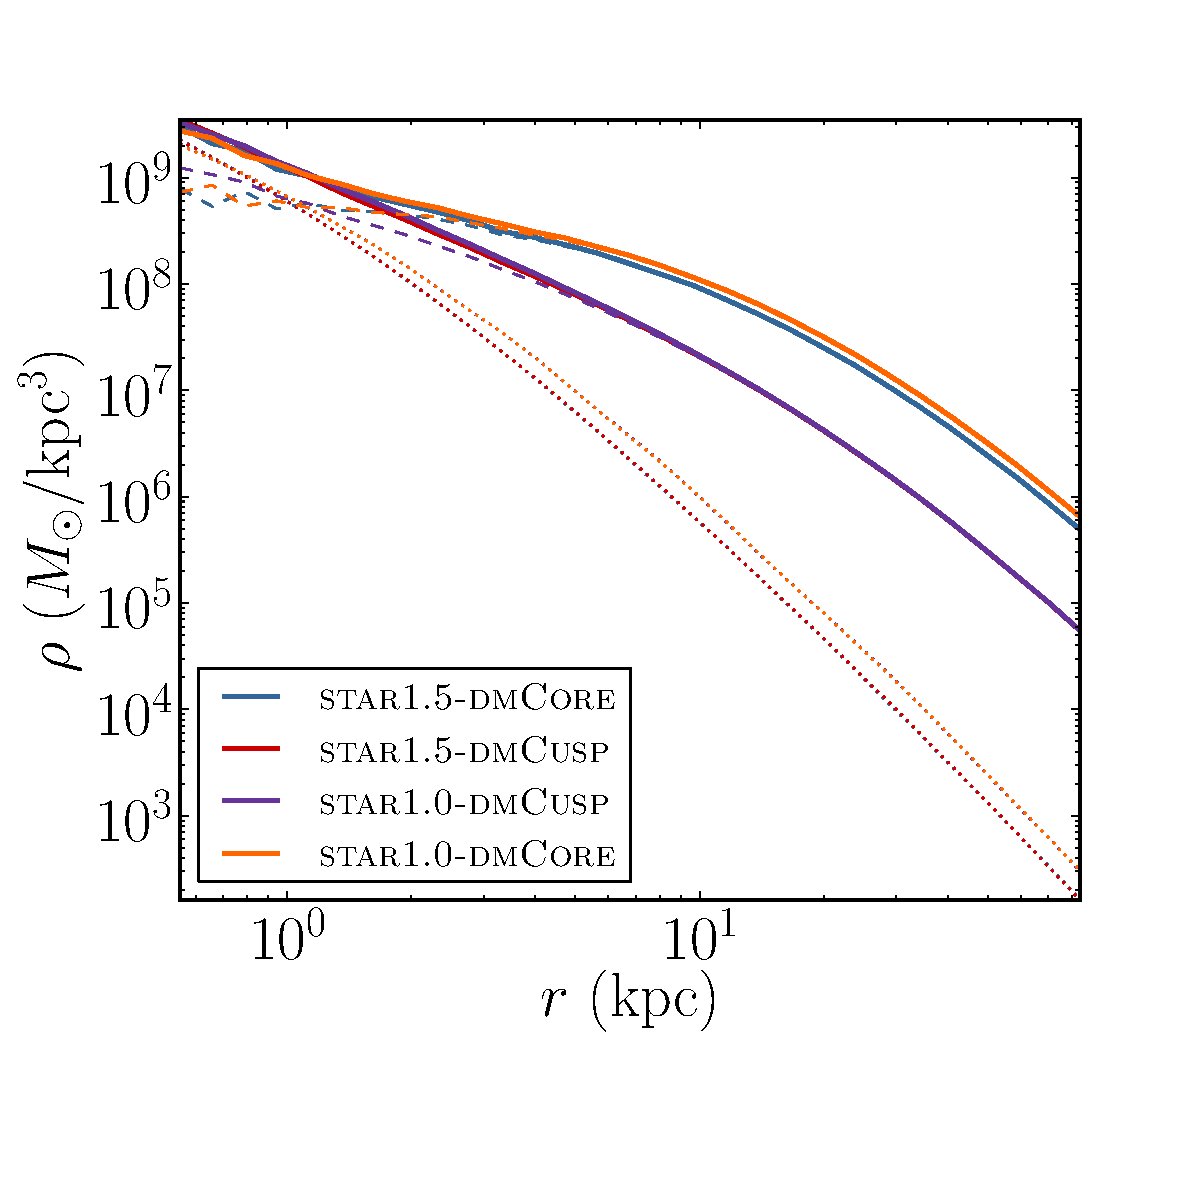
\includegraphics[width=0.33\textwidth]{MockGalProfile-a.pdf} 
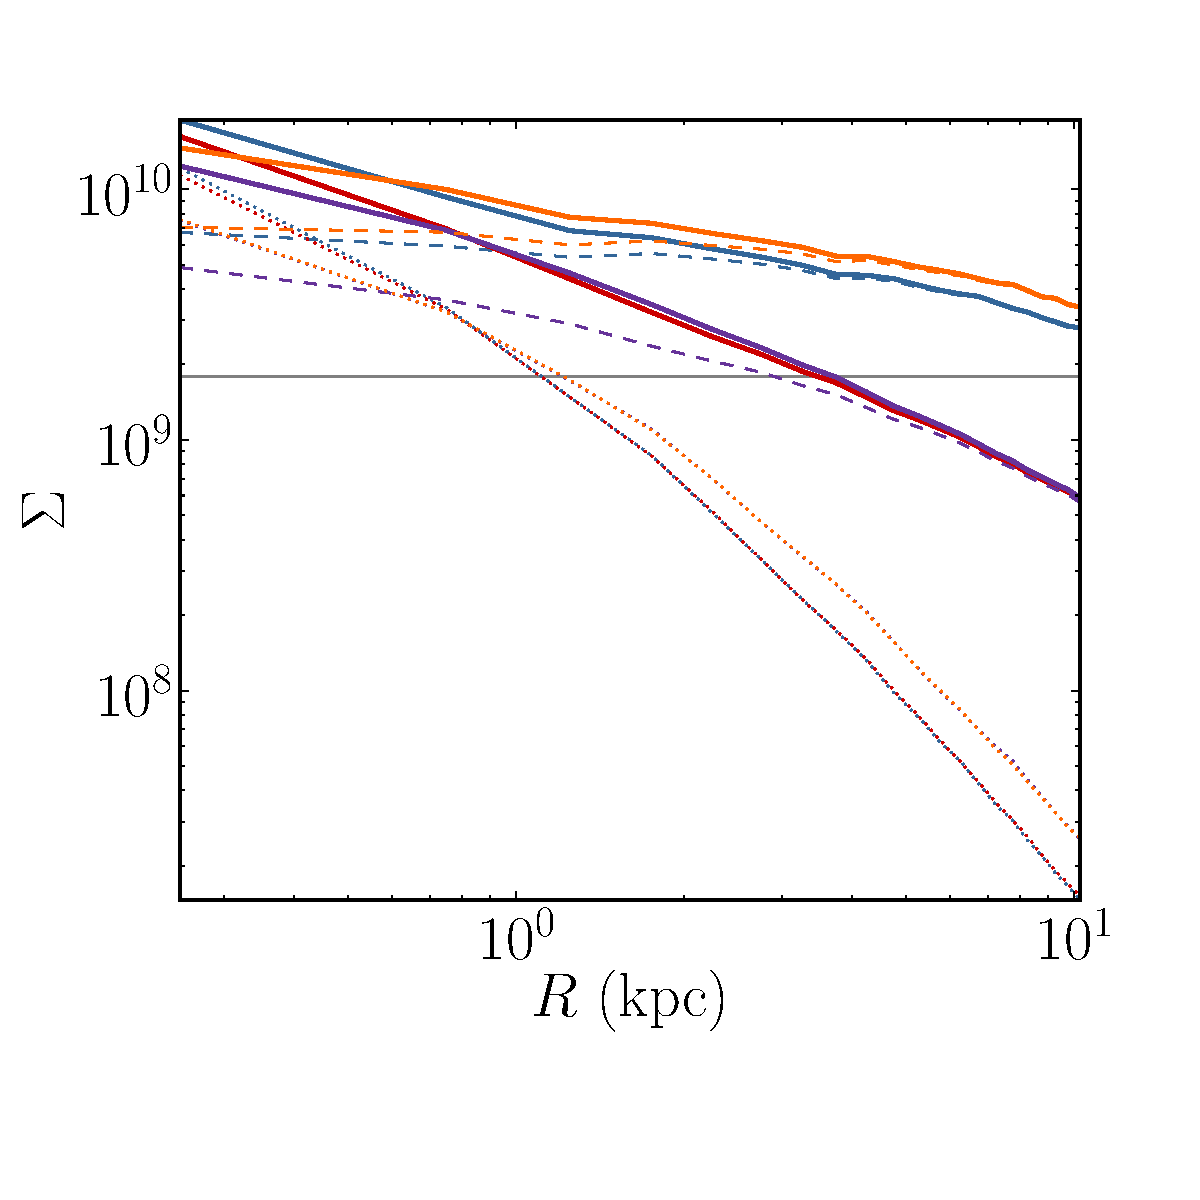
\includegraphics[width=0.33\textwidth]{MockGalProfile-b.pdf} 
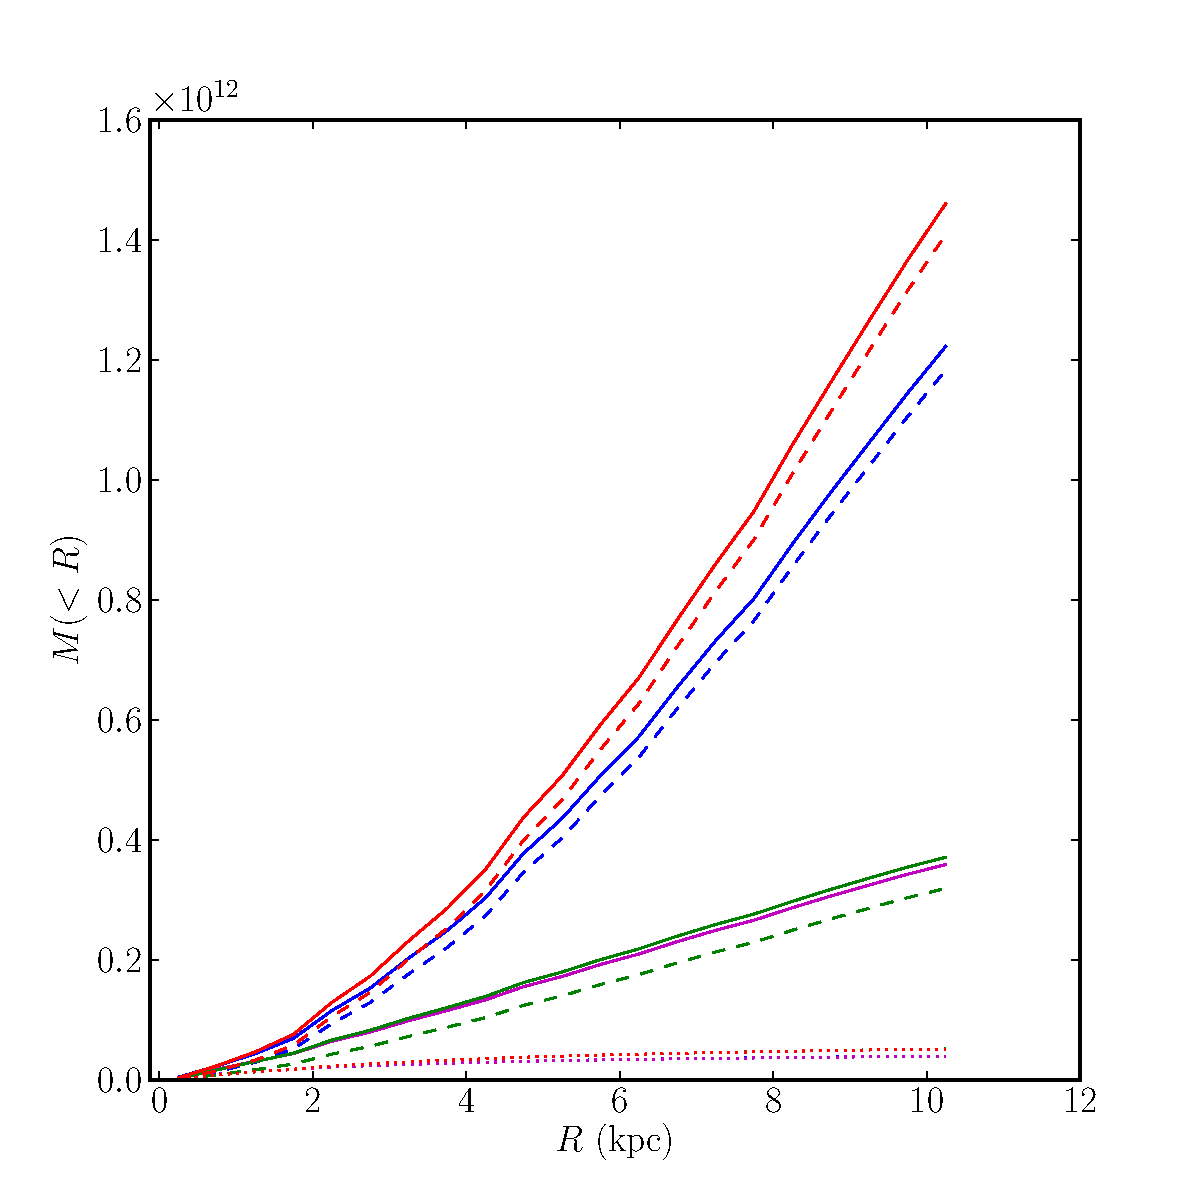
\includegraphics[width=0.33\textwidth]{MockGalProfile-c.pdf}
\caption{{\bf JR. Cut the analytic profiles from this Figure. All fonts and labels should be larger. Left panel should start at 0.7kpc.}
\textbf{Left:} 
Density averaged in spherical shells of the four galaxy mocks: AA, AC, BB and BC, showing the stellar (dotted), dark matter (dashed),
and total (solid) densities, respectively. Notice that the stars in models BB and BC contribute significantly to the central potential. 
\textbf{Middle:} 
The radially averaged two-dimensional projected density.
The critical density for lensing at $z_L=0.31$, $\kappa_\mathrm{crit}\sim 1.8\e{9}$\Msun/kpc$^2$, is marked by the horizontal line. 
\textbf{Right:}
The enclosed projected mass.
}
\label{mock galaxies}
\end{figure*}

In \figref{mock galaxies}, we show the 3D radial density, 
the 2D projected density, and the 2D enclosed mass for each
galaxy.

\subsection{Lens configurations}\label{sec:lensconfig} %--------------------------------------------------------------

For each of the four galaxies, we used the raytracing feature of \Glass\
described in \secref{Raytracing} to construct 12 lensing scenarios {\bf JR. We have 12 lensing scenarios, but only 6 panels in Figure 2. Is this number correct?}:

\begin{enumerate}
\item one double and one extended double;
\item one quad and one extended quad;
\item two 2-source quads with varying redshift contrast.
\end{enumerate}
The `extended' configurations use multiple point sources at the same redshift to simulate an extended source (that will produce an arc-like image). \figref{arrival surfaces} shows the configuration for the extended quad, along with the other cases. 

\begin{figure*}
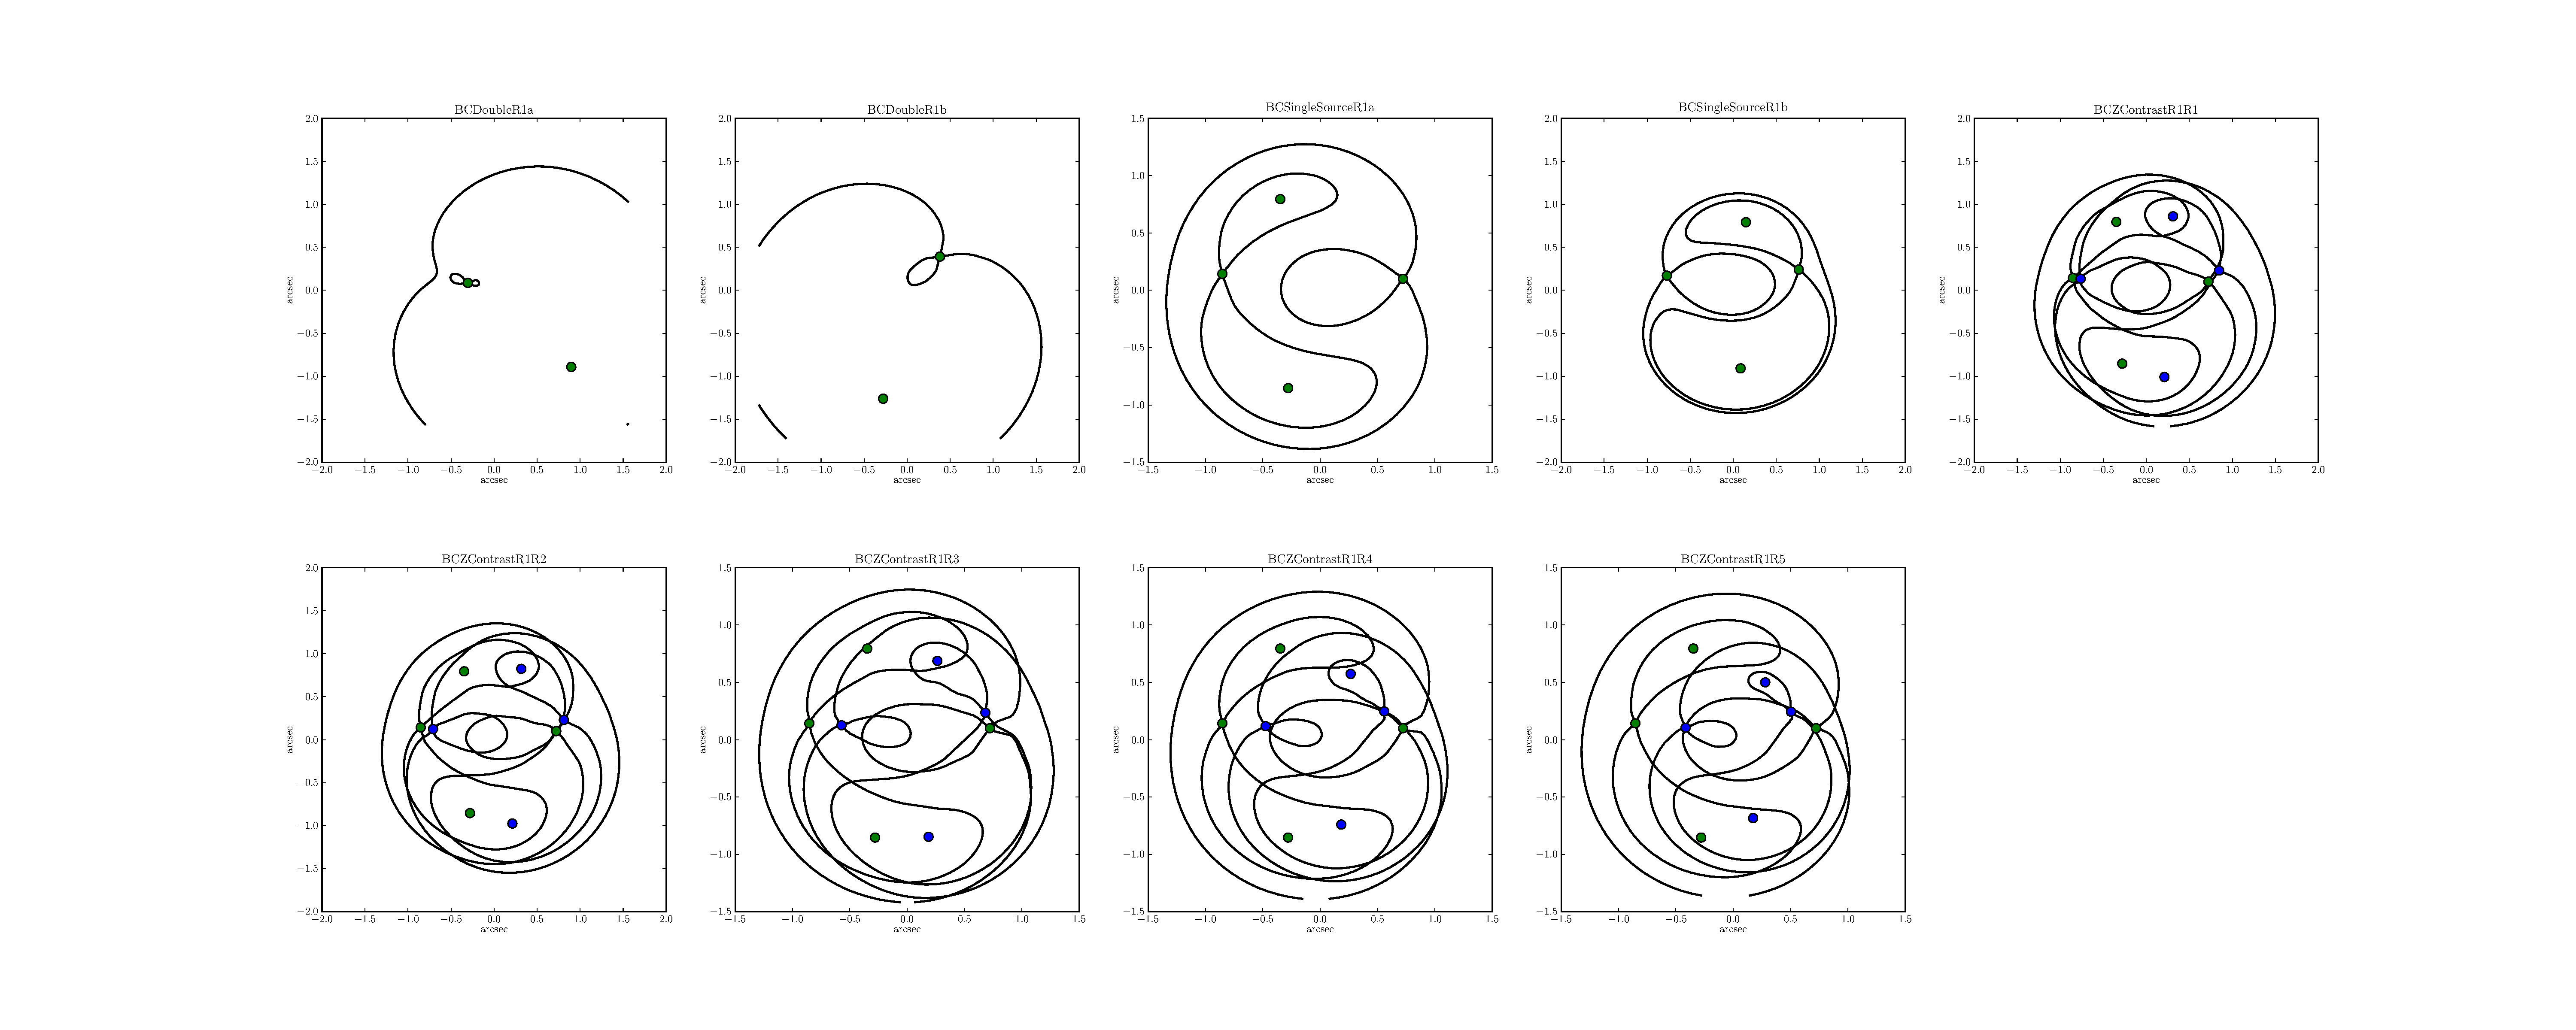
\includegraphics[width=0.85\textwidth]{BCarrival_surfaces}
\caption{The lens configurations for the six test cases using the BC mock galaxy. Here,
the central image is shown, although not all tests include it. The central image belongs
to only one set of images to avoid overconstraining the models. Similar colors group
images that share a common source. In the case of the extended image systems the source
is at the same redshift, while the redshift is varied between the systems in the 
ZConstrast cases. Grey circles are a visual aid to help determine radial separation
between images. The axes are measure in arcseconds.}
\label{arrival surfaces}
\end{figure*}

Each of these configurations were modelled with and without time delays and with
and without a central image. (The central image is typically highly demagnified. For galaxy lenses it is very difficult to find since it lies along the sight line to the bright lensing galaxy; in clusters, however, such images have been seen (CITES)). We assumed for all our tests that the lensing mass
was radially symmetric ({\bf JR. Need to better-define this symmetry here.}. For our mock data, this is known to be true; it is
most often the case with real galaxies, unless there is an obvious observed
asymmetry. The central pixel was refined into a further nine pixels to capture
any steep rise in the profile. Two of the four mock galaxies have a steeply rising
inner profile. {\bf JR. What happens if we don't assume this symmetry? We ought to add an appendix showing this for one example case.}

\section{Results}\label{sec:results}
\figref{reconstruction} shows a typical reconstruction of a
lens. The far left plot shows the ensemble average arrival time surface with
image marked as circles and the inferred source position as a diamond. The
center plot shows the radial density profile. The error bars cover the full
range of models generated by \Glass {\bf JR. Why do this? Surely 1 or 2 sigma errors make more sense? I've deleted the ``full ensemble" results and kept the $1\sigma$ ones instead.}. The true density profile from the mock
data is also plotted for comparison. The vertical lines mark the radial
position of the images. The final plot on the right is of the enclosed mass. As
expected, the error bars are smallest in the region of the images where the most
information about the lens is present. The dip in the profile at the end of the
profile is due to the cut off in mass in the lensing map. This is of little
importance, though, as there is no lensing information there.

\begin{figure*}
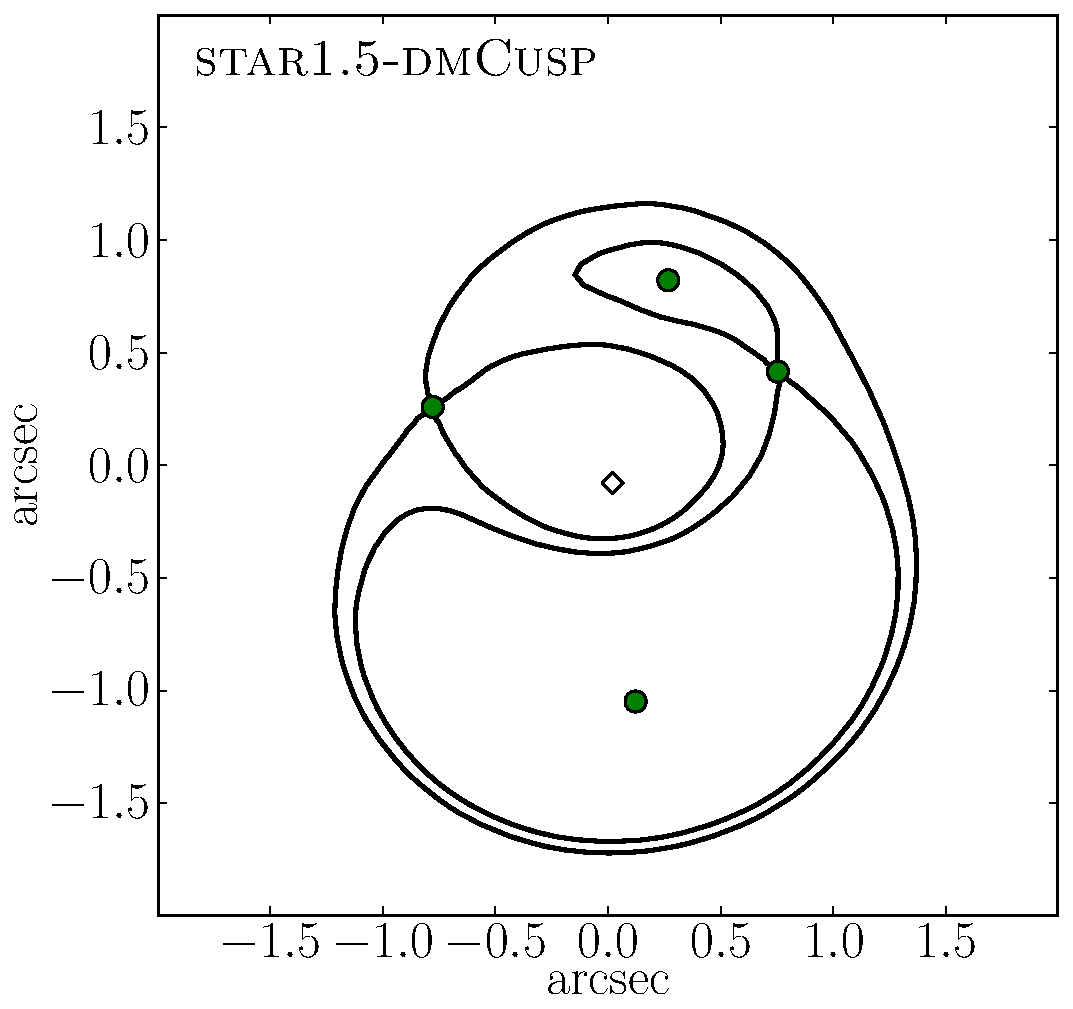
\includegraphics[width=0.33\textwidth]{BCQuadR1a_TmS-a.pdf}
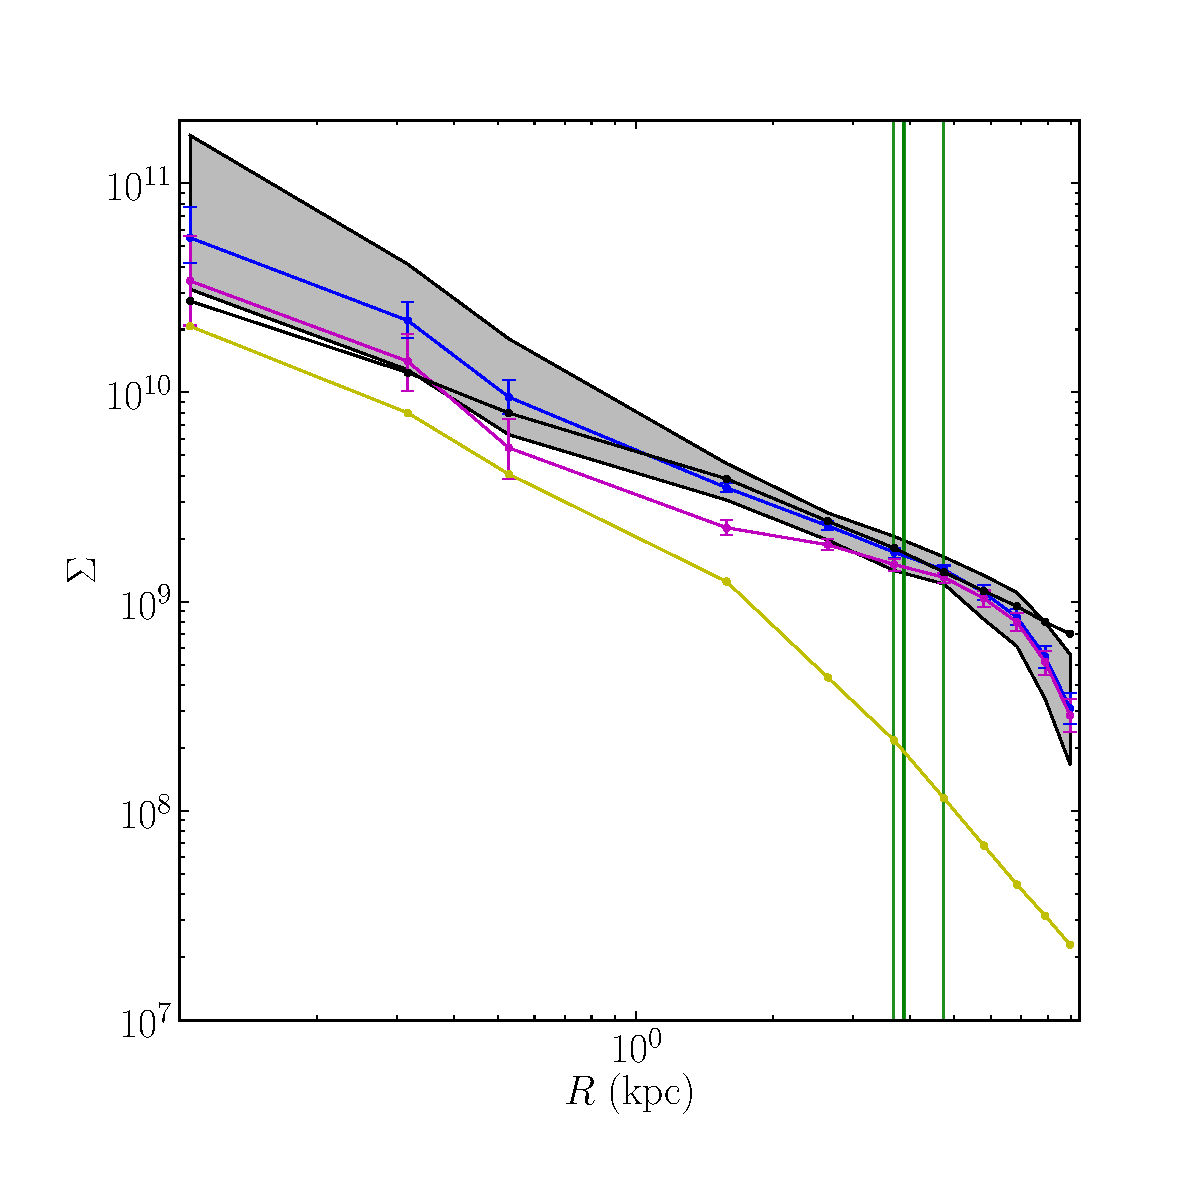
\includegraphics[width=0.33\textwidth]{BCQuadR1a_TmS-b.pdf}
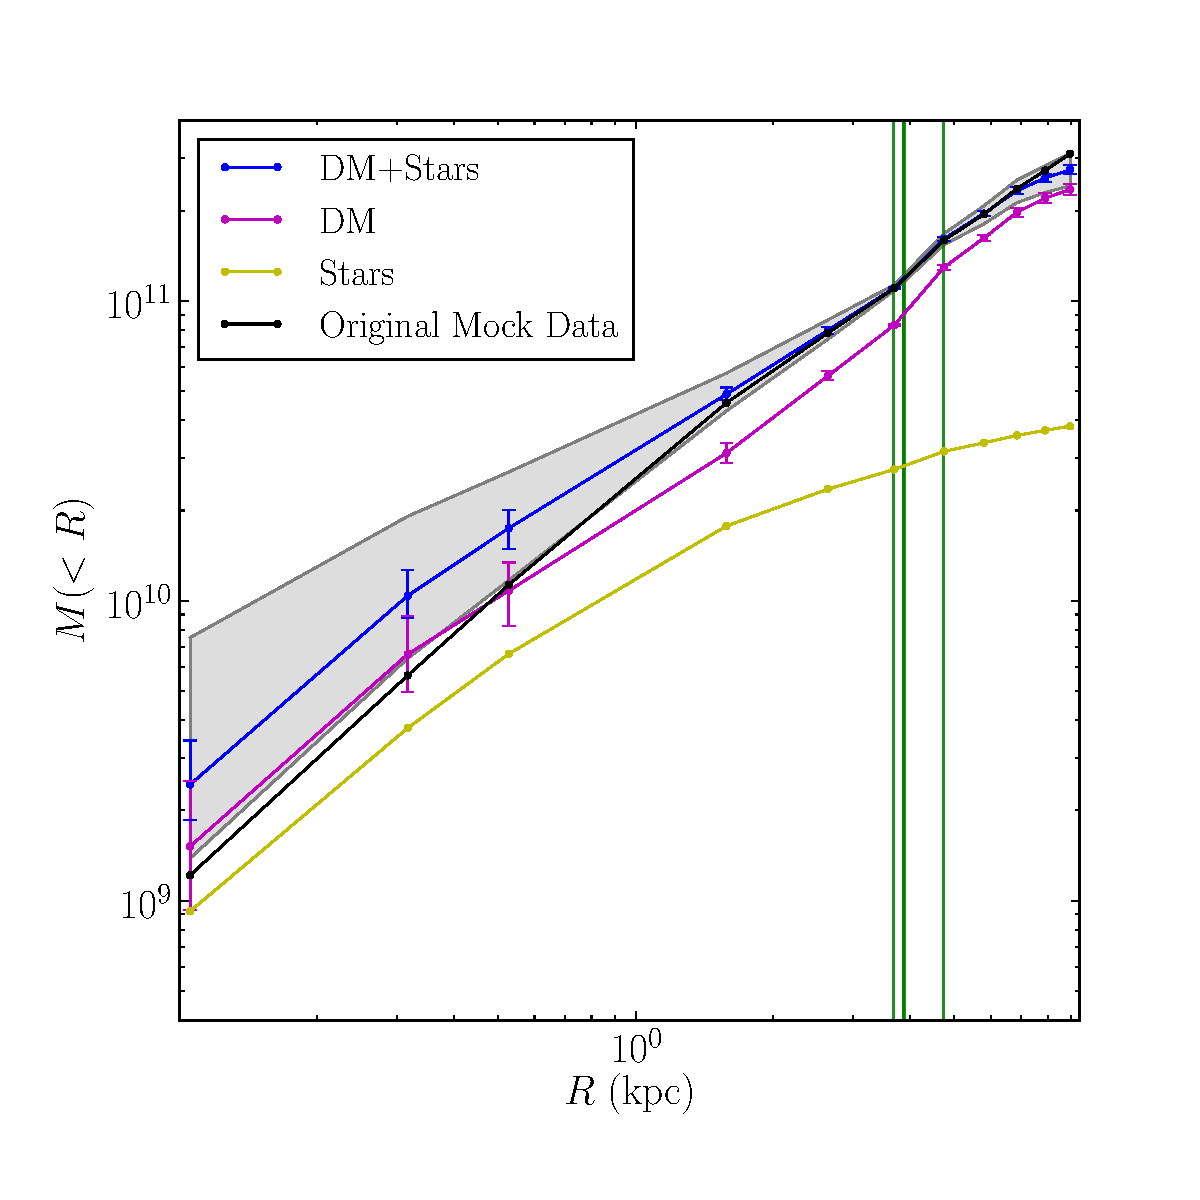
\includegraphics[width=0.33\textwidth]{BCQuadR1a_TmS-c.pdf}
\caption{
{\bf JR. Need to homogenise plot dimensions here. Larger fonts as in Figure 1 are also required.} 
A typical reconstructed lens. Here we present results for a single quad image lensed by the BC mock galaxy.
\textbf{Left:}
The arrival time surface. 
\textbf{Middle:}
The surface density. The magenta curve represents the dark matter component,
the yellow curve the stellar component, and the blue curve is the sum of the two.
The black curve comes from the original mass model used to create the lens.
The green vertical lines mark the radial positions of the images. The higher
resolution feature of \Glass\ has been used on the central pixel allowing the
steep profile to be captured.
\textbf{Right:}
The cumulative mass.}
\label{reconstruction}
\end{figure*}

The main results from modelling these different configuration are shown in black in
\figref{main results}. Each subplot corresponds to a different galaxy and
the vertical axis shows the range of `quality' of recovery, defined as: 
%
\begin{equation}
  \chi_i \equiv 100 \times \sqrt{\frac{\int_r (\rho_{\M_i}(r) - \rho_G(r))^2}{\int_r \rho_G(r)^2}}
  %\chi_i = \frac{\sum_r (\rho(r)_{\M_i} - \rho(r)_G)^2}{\sum_r \rho(r)_G^2}
\end{equation}
where $\rho_{\M_i}(r)$ is the recovered density profile for a mock model $\M_i$; and $\rho_G(r)$ is the true density profile. 

\begin{figure*}
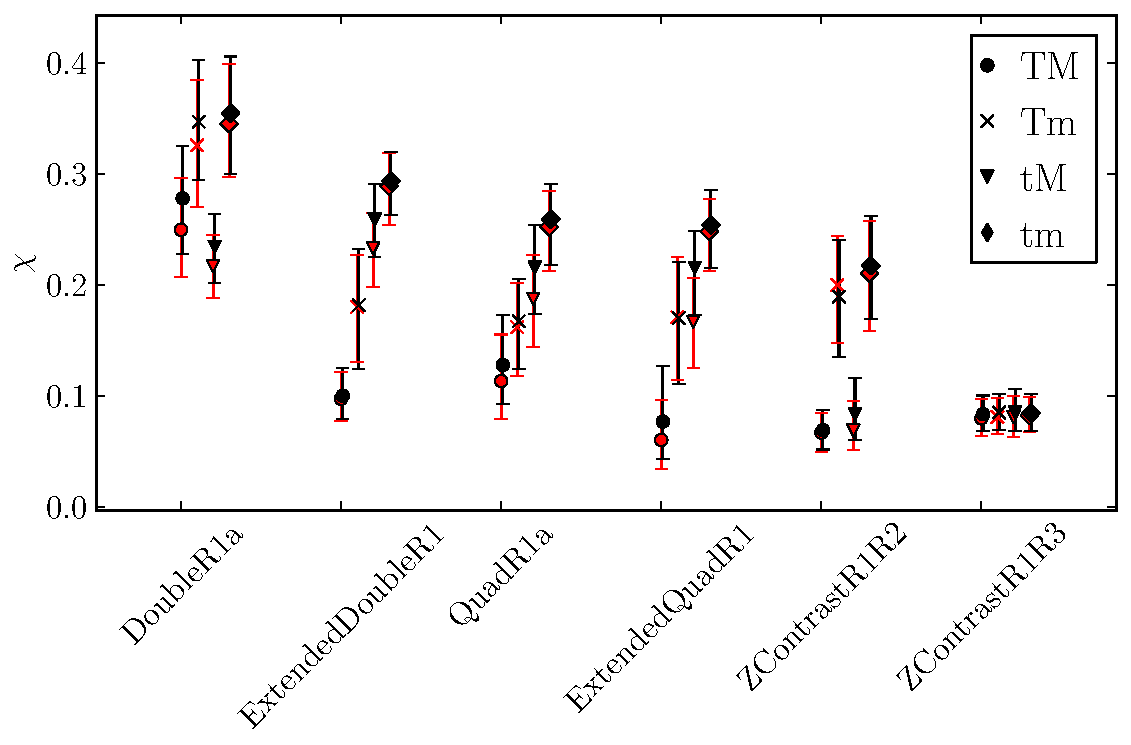
\includegraphics[width=0.49\textwidth]{AAchi2_profile.pdf}
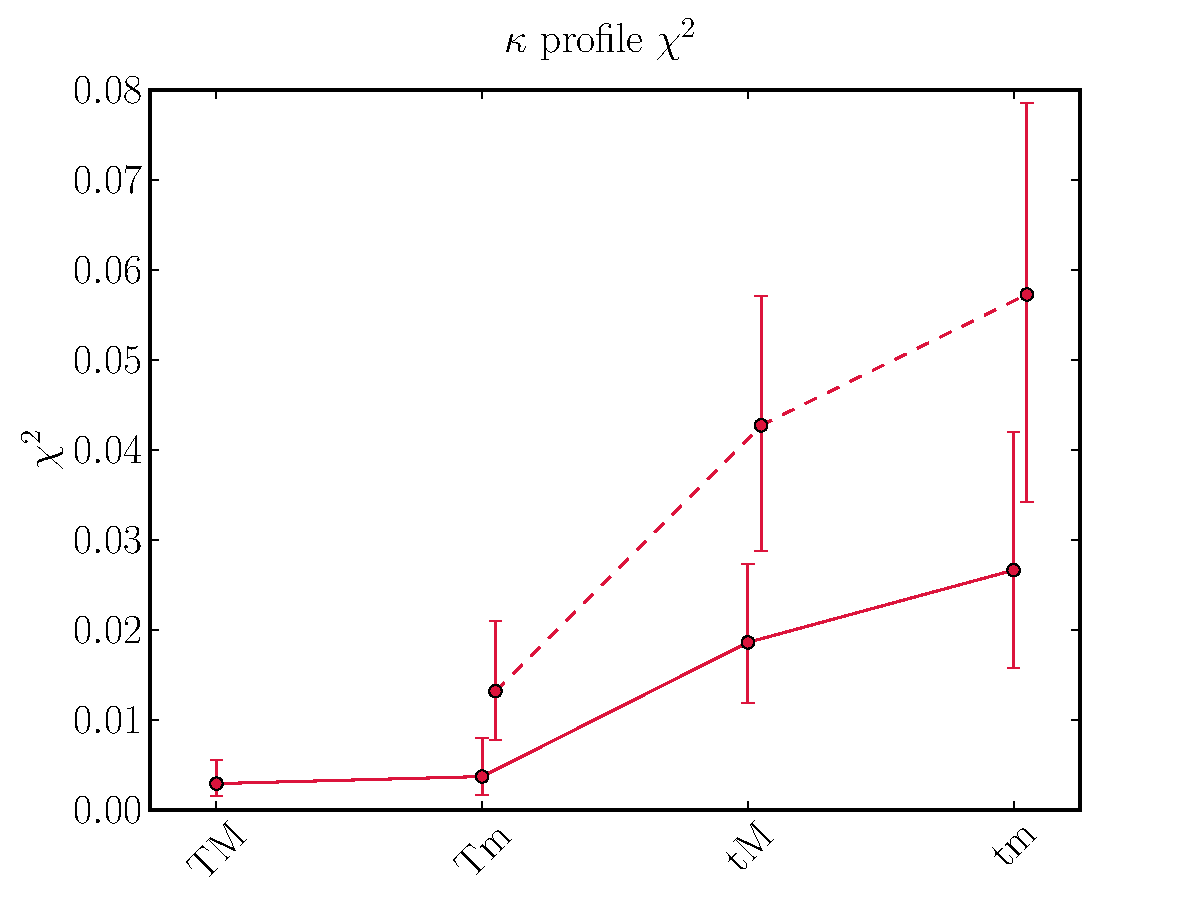
\includegraphics[width=0.49\textwidth]{BBchi2_profile.pdf}\\
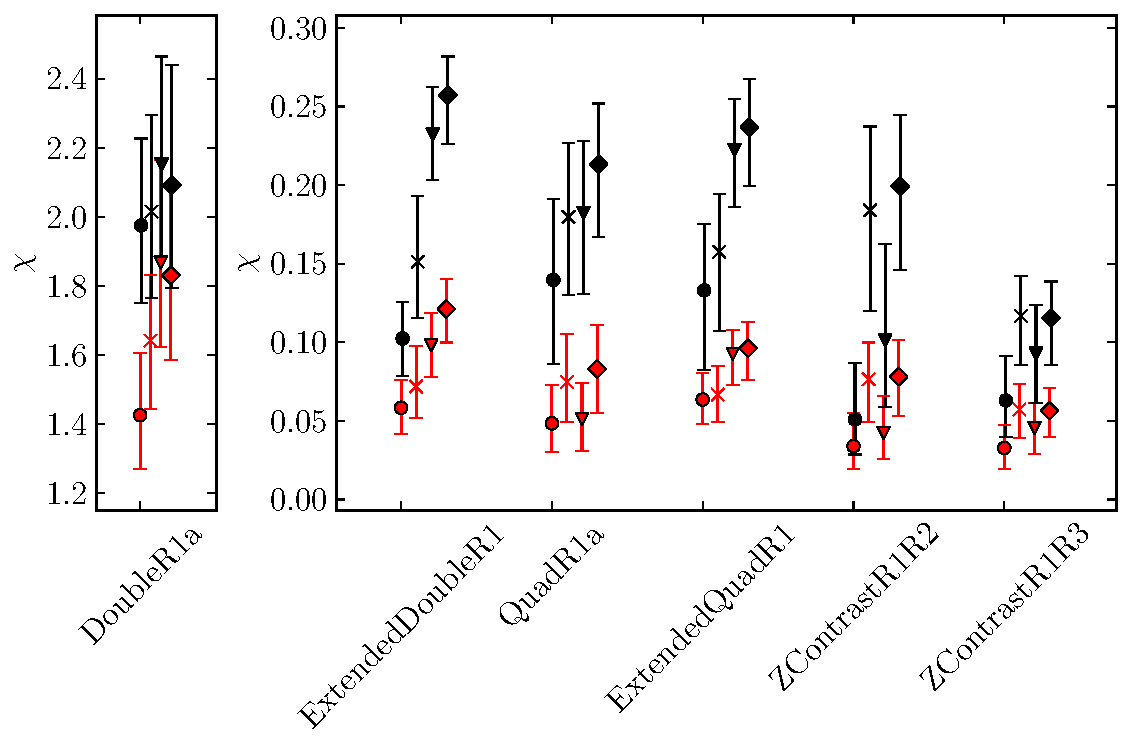
\includegraphics[width=0.49\textwidth]{ACchi2_profile.pdf}
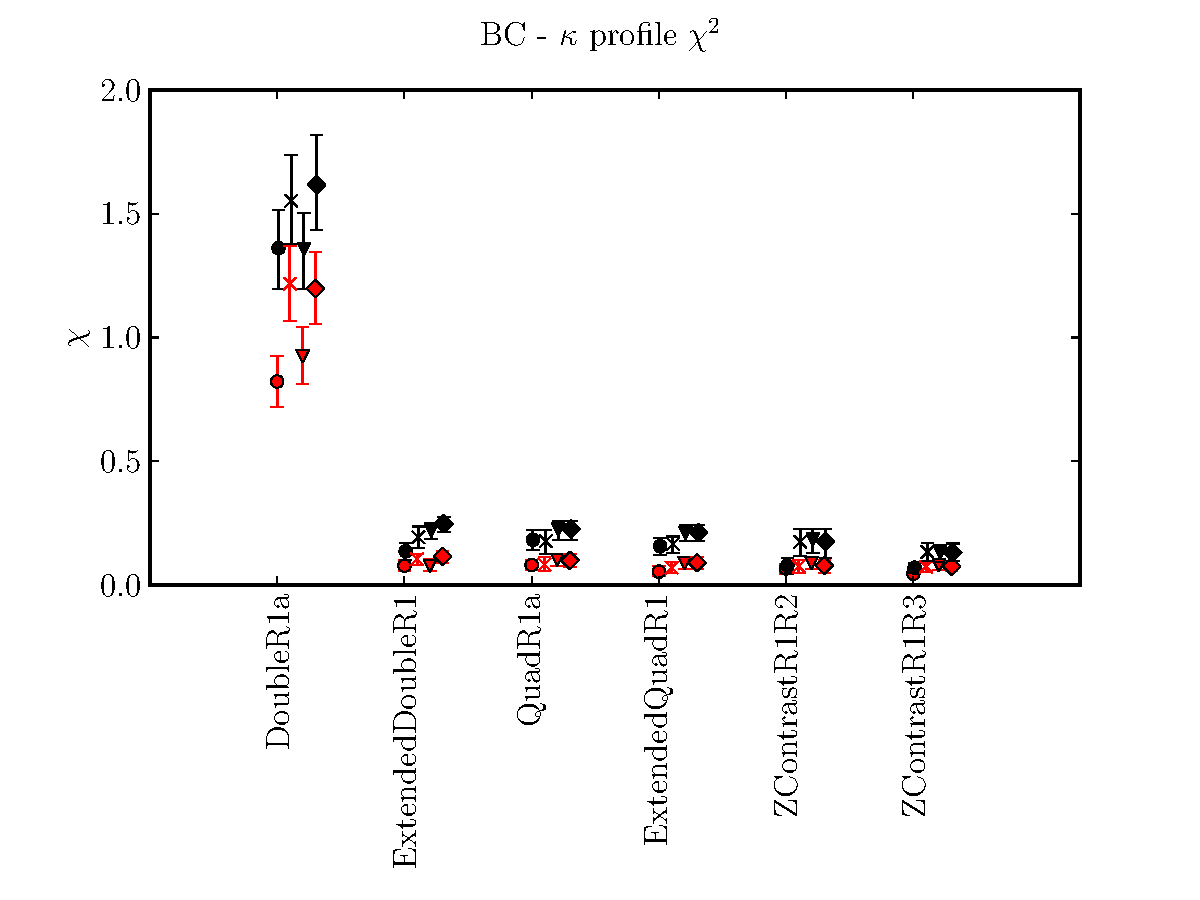
\includegraphics[width=0.49\textwidth]{BCchi2_profile.pdf}
\caption{The main results showing the quality of model recovery. Each panel corresponds to 
the named mock galaxy, whose parameters are listed in \tabref{mock galaxy params}. Within
each panel are six groups of results for each of six lens morphologies. Each morphology
considered the presence of time delays and a central image. The black markers are for tests
that did not include the stellar mass as a lower bound constraint, while the red markers
indicate where the stellar mass has been given. Error bars show the $1\sigma$ equivalent interval sampled from the model ensemble.}
\label{main results}
\end{figure*}

\begin{figure*}
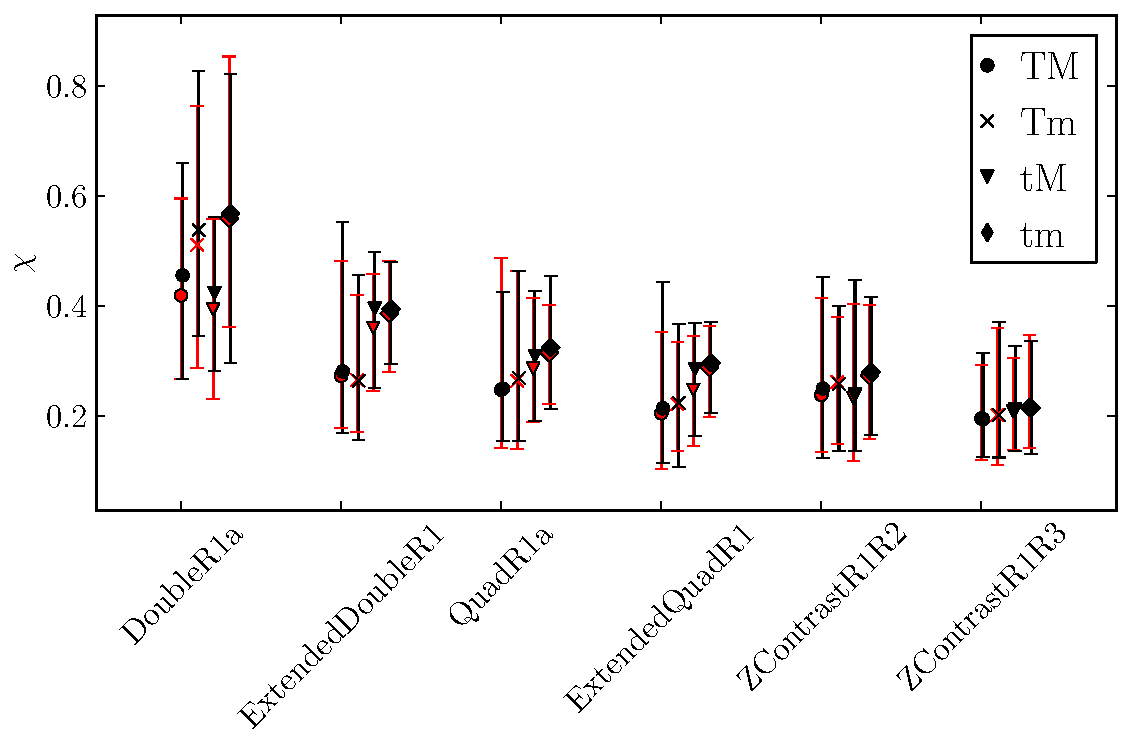
\includegraphics[width=0.49\textwidth]{AAchi2-full.pdf}
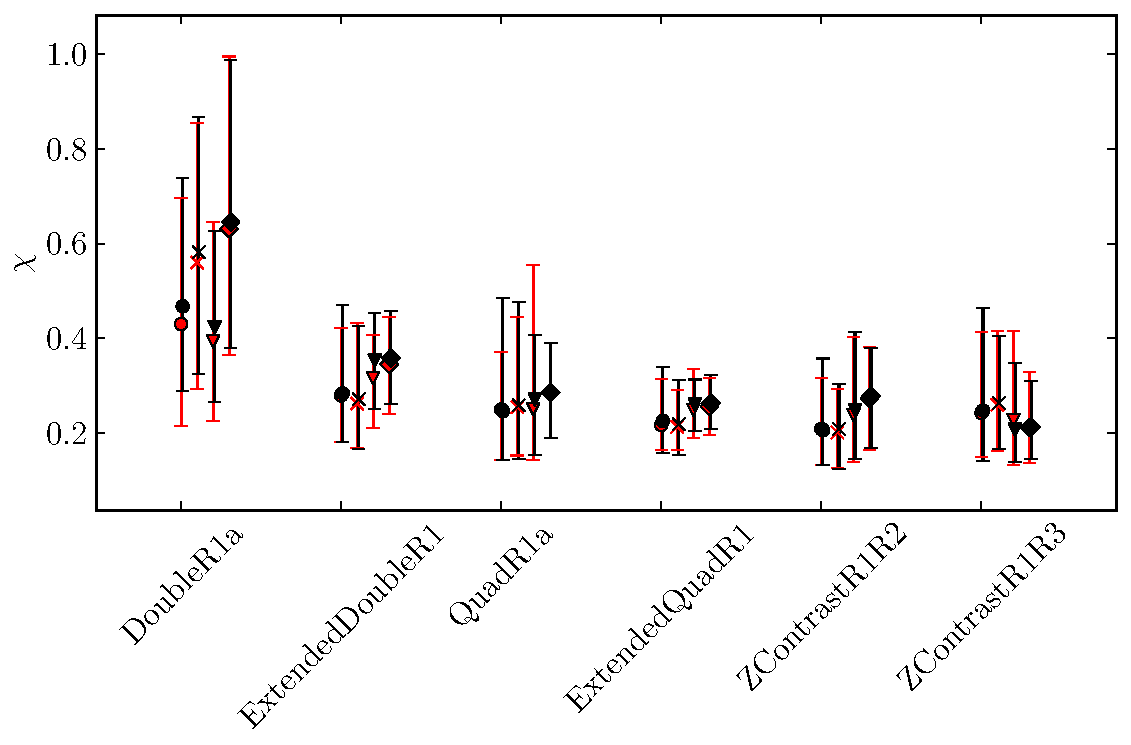
\includegraphics[width=0.49\textwidth]{BBchi2-full.pdf}\\
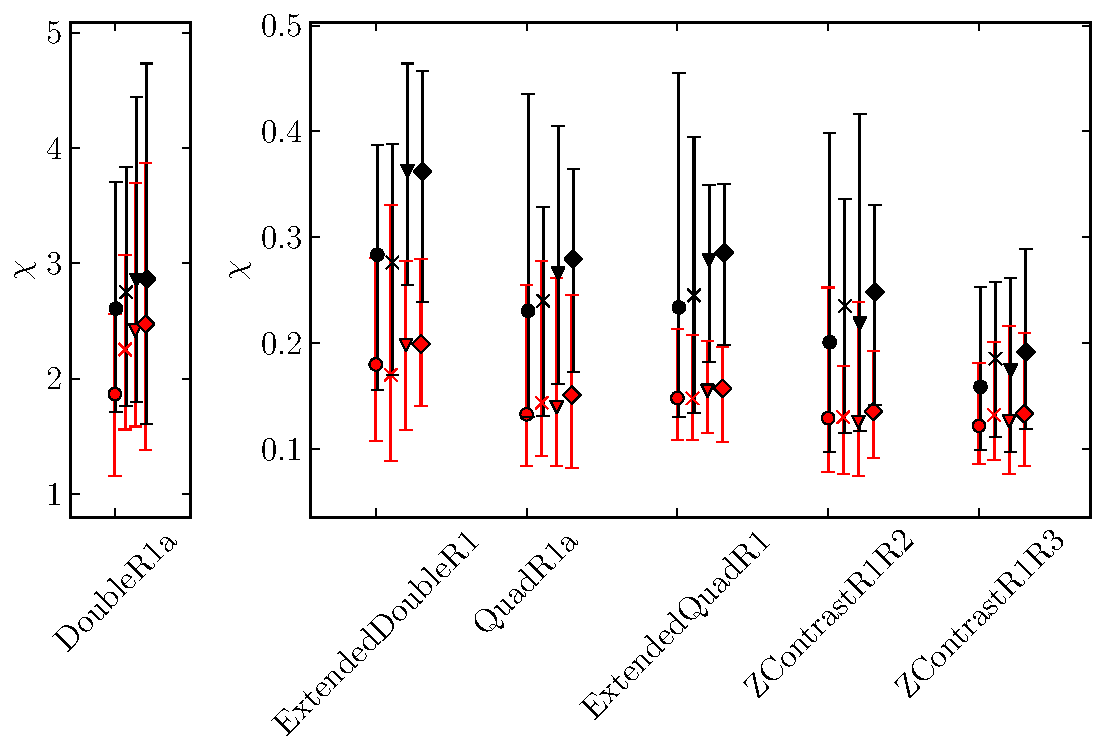
\includegraphics[width=0.49\textwidth]{ACchi2-full.pdf}
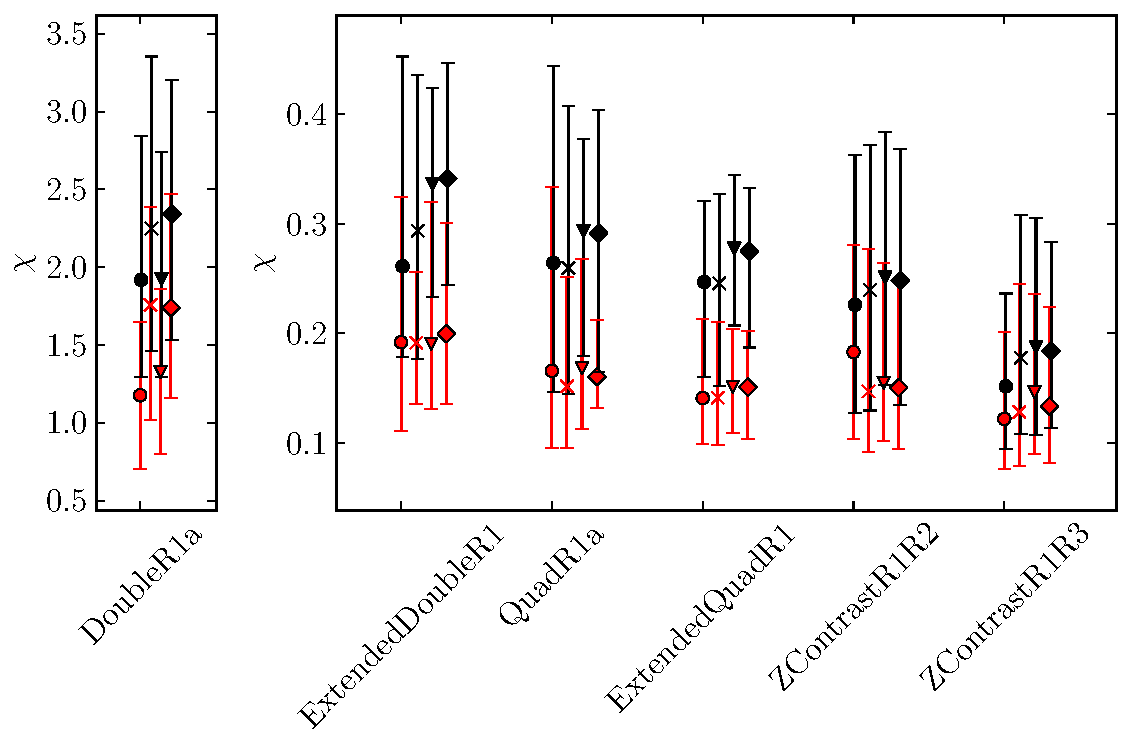
\includegraphics[width=0.49\textwidth]{BCchi2-full.pdf}
\caption{{\bf JR. This should be also with $1\sigma$ errors. Also need to do this plot for Claudio's shape measure.} Pixel-wise $\chi$.}
\label{main results pixel-wise}
\end{figure*}

The abundance of strong lensing data increases from left to right within each plot. As
a result, there is a general trend for the reconstruction quality to increase
(and for $\chi$ to decrease). By adding more measurable information to each
configuration the quality can also be affected. When both time delays and a
central image are present the quality is highest. A double is known to provide
very little constraint on the mass distribution. This is particularly evident in
galaxies AC and BC where the mass profile is steepest and the reconstruction of
the double is poorest. However, the addition of an arc is sufficient to correct
this.

\subsection{Stellar mass}
\label{stellar mass}

The stellar mass distribution gives a lower bound on the total mass. Where the stars dominate the central potential, it can provide a powerful constraint extra to the strong lensing data. We took the stellar mass directly from
the generated galaxies and projected the particles onto the pixels. \Glass\
also offers an option to interpolate any map of stellar mass (e.g., from an
observation) onto the pixels. The linear constraint is added to \Glass\ by
writing $\kappa_n = \kappa_{dm,n} + \kappa_{s,n}$ as the sum of the
dark matter and stellar mass components in the potential (\eqnref{discrete
potential}). Since each $\kappa_{s,n}$ is just a constant we do not add new,
separate equations for each pixel. Although we assume a perfect recovery of the stellar mass here, it is straightforward to add errors as the stellar mass constraint remains linear: $\kappa_n = \kappa_{dm,n} + \epsilon \kappa_{s,n}$, where $\epsilon \sim 1$ is an additional error parameter. 

With the stellar mass lower bound, the improvement of the reconstruction
quality shown in \figref{main results} is quite dramatic for the
steepest mock galaxies (AC and BC). This is because these models are dominated
by stars in the inner region. By contrast, the other two galaxies -- where the stars contribute negligibly to the potential -- are unaffected.

\subsection{Stellar kinematics}\label{sec:results_stellar_kinematics}

As outlined in \S\ref{sec:glass}, \Glass\ can also run post processing
routines on the model ensemble which can be used to apply non-linear constraints. As an example, we consider here constraints from stellar kinematics. The models in the \Glass\ ensemble are processed as described in \S\ref{sec:glasskinematics}. To illustrate the power of stellar kinematic constraints, in
\figref{sigma-beta}, we plot the projected velocity dispersion calculated for one model model (extracted from the full ensemble) of the BC Quad with time delays and stellar mass (left), and the mean projected velocity dispersion (\eqnref{eqn:virialaverage}) as a function of the upper limit of the averaging integral (the aperture size), $a_p$ (right). In both cases, we calculate curves for two extrema velocity anisotropies: $\beta=0$ (green) and $\beta=1$ (red). Over-plotted is the correct answer for the BC model (black). The stellar half mass radius (yellow) Einstein radius (black) are marked by vertical lines. For this configuration, these two radii are well-separated.

Without even sweeping through the model ensemble and formally accepting/rejecting models, \figref{sigma-beta} already illustrates what we can hope to obtain from stellar kinematics. The most robust constraints follow if we can integrate out the effect of $\beta$ (right panel), since this is difficult to measure. For large enough aperture size ($a_p > 2r_{1/2}$), the average projected dispersion converges on a single well defined value independently of $\beta$. Since this converged value follows from the virial theorem, it is also rather insensitive to the shape of the potential \citep{2012ApJ...754L..39A}: it constitutes a robust constraint on the lensing potential. On the other hand, if the mass profile is well-constrained already at $r \sim r_{1/2}$, then we can use stellar kinematics to probe $\beta$. This can be seen in the left panel of \figref{sigma-beta}. Here we see that for a well-constrained mass model, the $\beta = 1$ curve lies significantly off from the true answer that has $\beta(r) \sim 0$. 

We now consider formally accepting/rejecting models from the full ensemble. We consider two regimes of interest: a model with a double where the mass profile is poorly constrained (XXX), and a model where the mass profile is very well constrained by the lens data (YYY). In the former case, we use $\overline{\sigma}(2 r_{1/2})$ to probe the mass independently of $\beta(r)$. We accept/reject models assuming a Gaussian error on measured $\overline{\sigma}(2 r_{1/2})$ of $\pm 10$\,km/s (similarly to the data quality presented for example in \citealt{2002MNRAS.337L...6T}). The results are shown in \figref{main results}, blue data points. In the latter case, we ask whether the data favour $\beta = 0$ or $\beta = 1$ by obtaining a $\chi^2$ goodness of fit measure between the true and modelled $\sigma_p(R)$. We accept/reject models from the ensemble above. The results for $\beta$ are shown in Figure ZZZ. 

The results for stellar kinematics match our expectations from \S\ref{sec:kinematics}. Where the lens data already constrain the mass distribution at $r \sim r_{1/2}$, stellar kinematics provide valuable information about the velocity anisotropy of the stars, $\beta$ (see Figure ZZZ). Where the lens data poorly constrain the mass distribution at $r_{1/2}$, we may `integrate out' the effect of unknown $\beta$ to obtain a robust measure of $M(r_{1/2})$ from the stellar kinematics. This latter is robust to both uncertainties in $\beta(r)$ and to our assumption of spherical symmetry in the kinematic models \citep{2012ApJ...754L..39A}. Finally, we note that there is a third interesting case. If the lens models well-constrain $M(r_{1/2})$ and stellar kinematics are available, then these can be used to probe cosmological models (see \S\ref{sec:theory}). We explore this in more detail in a separate publication. 

\begin{figure*}
\includegraphics[width=0.49\textwidth]{BCQuadR1a_TmS-sb.pdf}
\includegraphics[width=0.49\textwidth]{BCQuadR1a_TmS-sb.pdf}
\caption{{\bf Left:} {\bf JR. Jonathan to add.} The projected velocity dispersion calculated for one model model (extracted from the full ensemble) of the BC Quad with time delays and stellar mass. {\bf Right:} The mean projected velocity dispersion (\eqnref{eqn:virialaverage}) as a function of the upper limit of the averaging integral (the aperture size), $a_p$. In both cases, we calculate curves for two extrema velocity anisotropies: $\beta=0$ (green) and $\beta=1$ (red). Over-plotted is the correct answer for the BC model (black) {\bf JR. Jonathan to add}. The stellar half mass radius (yellow) Einstein radius (black) are marked by vertical lines. For this configuration, these two radii are well-separated.}
\label{sigma-beta}
\end{figure*}

%\subsection{Velocity dispersions}
%
%\begin{itemize}
%\item Can they predict radial profiles?
%\item Can we constrain lensing models from predicted velocity dispersions?
%\item Use a constructed spherical halo G2 following a $\rho \propto r^{-\gamma}$ profile with stellar halo same as G1.
%\item Vary $z$ of the halo, possibly orientation.
%\item Should be able to recover $\gamma$ very well.
%\item Use G1. Show problems with recovering $\gamma$.
%\end{itemize}

%\subsection{With/without time delays and central image} %--------------------------------------------------------------

%We also considered the effect of having time delays or a central image. The
%central image is usually highly demagnified and obscured by the lensing galaxy,
%but in clusters the central image is observable. In this case we can imagine
%the galaxies to be clusters since the problem is scale-free. A recontruction of
%AASingleQuadR1a\_Tm is shown in \figref{AASingleQuadR1a_Tm}. The suffix denotes
%which combination of time delays (T) and central image (M) was used. An
%uppercase letter indicates the feature is turned on, and a lowercase letter
%that it is turned off.

\section{Conclusions}\label{sec:conclusions}

{\bf JR. ACTION ITEMS.

\begin{enumerate} 

\item More references to be added to the introduction. Lots of work remains to be cited. Were we really the first to test lensing on N-body mocks? Perhaps for strong lensing, but certainly not for weak. 

\item Understand ``Schneider's degeneracy". Add reference/commentary accordingly. 

\item Prasenjit to write/finish section on stellar population synthesis modelling.

\item Jonathan to complete \S\ref{sec:glass}. Emphasise need for central adaptive grid. Add appendix showing convergence as Pixrad is increased. 

\item Jonathan to write section \S\ref{sec:glassextraimages} on removing models with extra images. 

\item Clarify amount of triaxiality (and the analytic density profile) in \S\ref{sec:mockdata}. 

\item Clarify number of lens configurations in \S\ref{sec:lensconfig}.

\item Add appendix showing how ``radial symmetry" prior affects results. Clarify meaning of this prior with a nice figure showing the symmetry. 

\item Show results for $1\sigma$ and $2\sigma$ rather than full \Glass\ ensemble. Add results for Claudio's shape measure. Discuss shape throughout results section and mention more explicitly in abstract and conclusions -- what quality of data do we need to robustly constrain the shape?

\item Add example plot of the projected density and recovered projected density (c.f. plots Jonathan made for my ERC proposal). 

\item Tidy up figures and other small items as detailed throughout -- see {\tt {\bf JR ... }}. 

\item Add accept/reject results for stellar kinematics (two figures) as detailed in \S\ref{sec:results_stellar_kinematics}. 

\end{enumerate} 
}


\appendix

\section{Raytracing convergence test}
Raytracing is sensitive to the map area and resolution set by $\Rmap$ and
$\Rpix$.  In the left panel of \figref{raytracing convergence tests} we compare
the change in time delays as we increase $\Rmap$.  The image system is a quad
with the central maximum image. When the projected mass begins to fall off the
time delays stabilize. In the right panel we see the effect of changing the
resolution of the map.  Increasing the resolution allows for more accurate
placement of the images and after about $\Rpix=40$ the image positions change
by less than 0.04 arcsec. The one image that continues to change is near to a
caustic.  

\begin{figure}
\plottwo{tdconv_pr45.pdf}{imgpos_conv_mr20.pdf}
\caption{(left) Test for predicted time delay convergence as $\Rmap$ changes.
$\Rpix=45$. After about $\Rmap=20$ most of the asymmetric mass is in the map.
(right) Test for predicted image position $\theta$ convergence as $\Rpix$
changes. $\Rmap=20$ arcsec.}
\label{raytracing convergence tests}
\end{figure}

\section{Derivation of pixelated density coefficients}
\label{Q derivation}
When the lens plane is pixelized we need a discrete form of the integral
%
\[\int \kappa(\vec\theta') \ln |\vec\theta-\vec\theta'| d^2\vec\theta' \]
%
In particular we want
%
\[\sum_n \kappa_n Q_n(\vec\theta)\]
%
where $Q_n$ is the logarithm evaluated over the $n$th pixel at position $\vec\theta_n = (x_n, y_n)$. Let the pixel side length be $a$.
Instead of working with a position vector $\vec\theta$ we work in cartesian coordinates such that
%
$|\vec\theta| = r = \sqrt{x^2 + y^2}$. The integral now becomes
%
\[Q_n(x,y) = \frac12 \int_{y_-}^{y_+}\int_{x_-}^{x_+} \ln (x'^2+y'^2) dx' dy'\]
%
where $x_\pm = x + x_n \pm (a/2)$ and similarly for $y_\pm$.
Using the identity
%
\[\int \ln(x^2+y^2) dx = x \ln(x^2+y^2) - 2x + 2y\arctan(x/a) \]
%
we can express $Q_n$ as the sum of four parts
%
\[Q_n(x,y) = \frac12 \left[ \tilde Q_n(x_+,y_+)
        + \tilde Q_n(x_-,y_-)
        - \tilde Q_n(x_-,y_+)
        - \tilde Q_n(x_+,y_-) \right]\]
%
where
%
\[\tilde Q_n(x,y) = xy(\ln r^2 - 3) + x^2\arctan(y/x) + y^2\arctan(x/y)\]

\section{Pixel resolution convergence test}
{\bf JR. Need to add an appendix showing convergence with increasing Pixrad.} 

\bibliographystyle{mn2e}
\bibliography{ms}

\end{document}

